\documentclass[11pt, a4paper]{article}

\usepackage[a4paper, margin=2cm]{geometry}
\usepackage{setspace}
\usepackage[portuguese]{babel}
\usepackage{graphicx}
\usepackage{hyperref}
\usepackage{amsfonts}
\usepackage[dvipsnames]{xcolor}
\usepackage{float}
\usepackage{footnote}
\usepackage{chngpage}

\chardef\_=`_

\onehalfspacing
\makesavenoteenv{tabular}

\title{\textbf{LI3 - Relatório da Fase II - Grupo 12}}
\author{
    Humberto Gomes (A104348) \\
    José Lopes     (A104541) \\
    José Matos     (A100612) \\
}
\date{janeiro de 2024}

\begin{document}

\maketitle
\setlength{\parskip}{\baselineskip}
\setlength{\parindent}{0pt}

\begin{abstract}
    Após a entrega da primeira fase deste trabalho, procurámos implementar as funcionalidades em
    falta para a conclusão do desenvolvimento desta aplicação: as restantes quatro \emph{queries},
    um modo de uso interativo (uma interface TUI), testes funcionais e de desempenho, e suporte
    para um \emph{dataset} de maior dimensão, mantendo um desempenho aceitável. Adicionalmente,
    procurámos também corrigir alguns aspetos do encapsulamento e da modularidade no nosso projeto.
\end{abstract}

\section{Estrutura do trabalho}

Nesta secção, procuramos descrever as diferenças entre a nossa arquitetura atual e a que tínhamos
na primeira fase do projeto. Devido ao elevado número de módulos, dividimos a aplicação em
subsistemas, que são descritos e esquematizados um a um, apresentados apenas com as relações de
dependência mais relevantes. Segue-se a nossa convenção gráfica:

\begin{itemize}
    \item Um retângulo com cantos arredondados representa uma estrutura de dados (entidade,
          gestor, alocador, \ldots);
    \item Um retângulo sem cantos arredondados representa um módulo cuja tarefa principal é a
          execução de código. Mesmo assim, alguns destes módulos podem conter estruturas de dados
          auxiliares (por exemplo, uma gramática definida no módulo de um \emph{parser});
    \item $A \rightarrow B$ significa que o módulo $A$ depende do módulo $B$.
    \item Nos subsistemas já existentes na primeira fase, um módulo ou relação de dependência
          representado(a) a {\color{ForestGreen}verde} indica que o(a) mesmo(a) estava ausente na
          entrega anterior.
\end{itemize}

\subsection{\emph{Parsing}}
\label{sec:parsing}

\begin{figure}[ht]
    \centering
    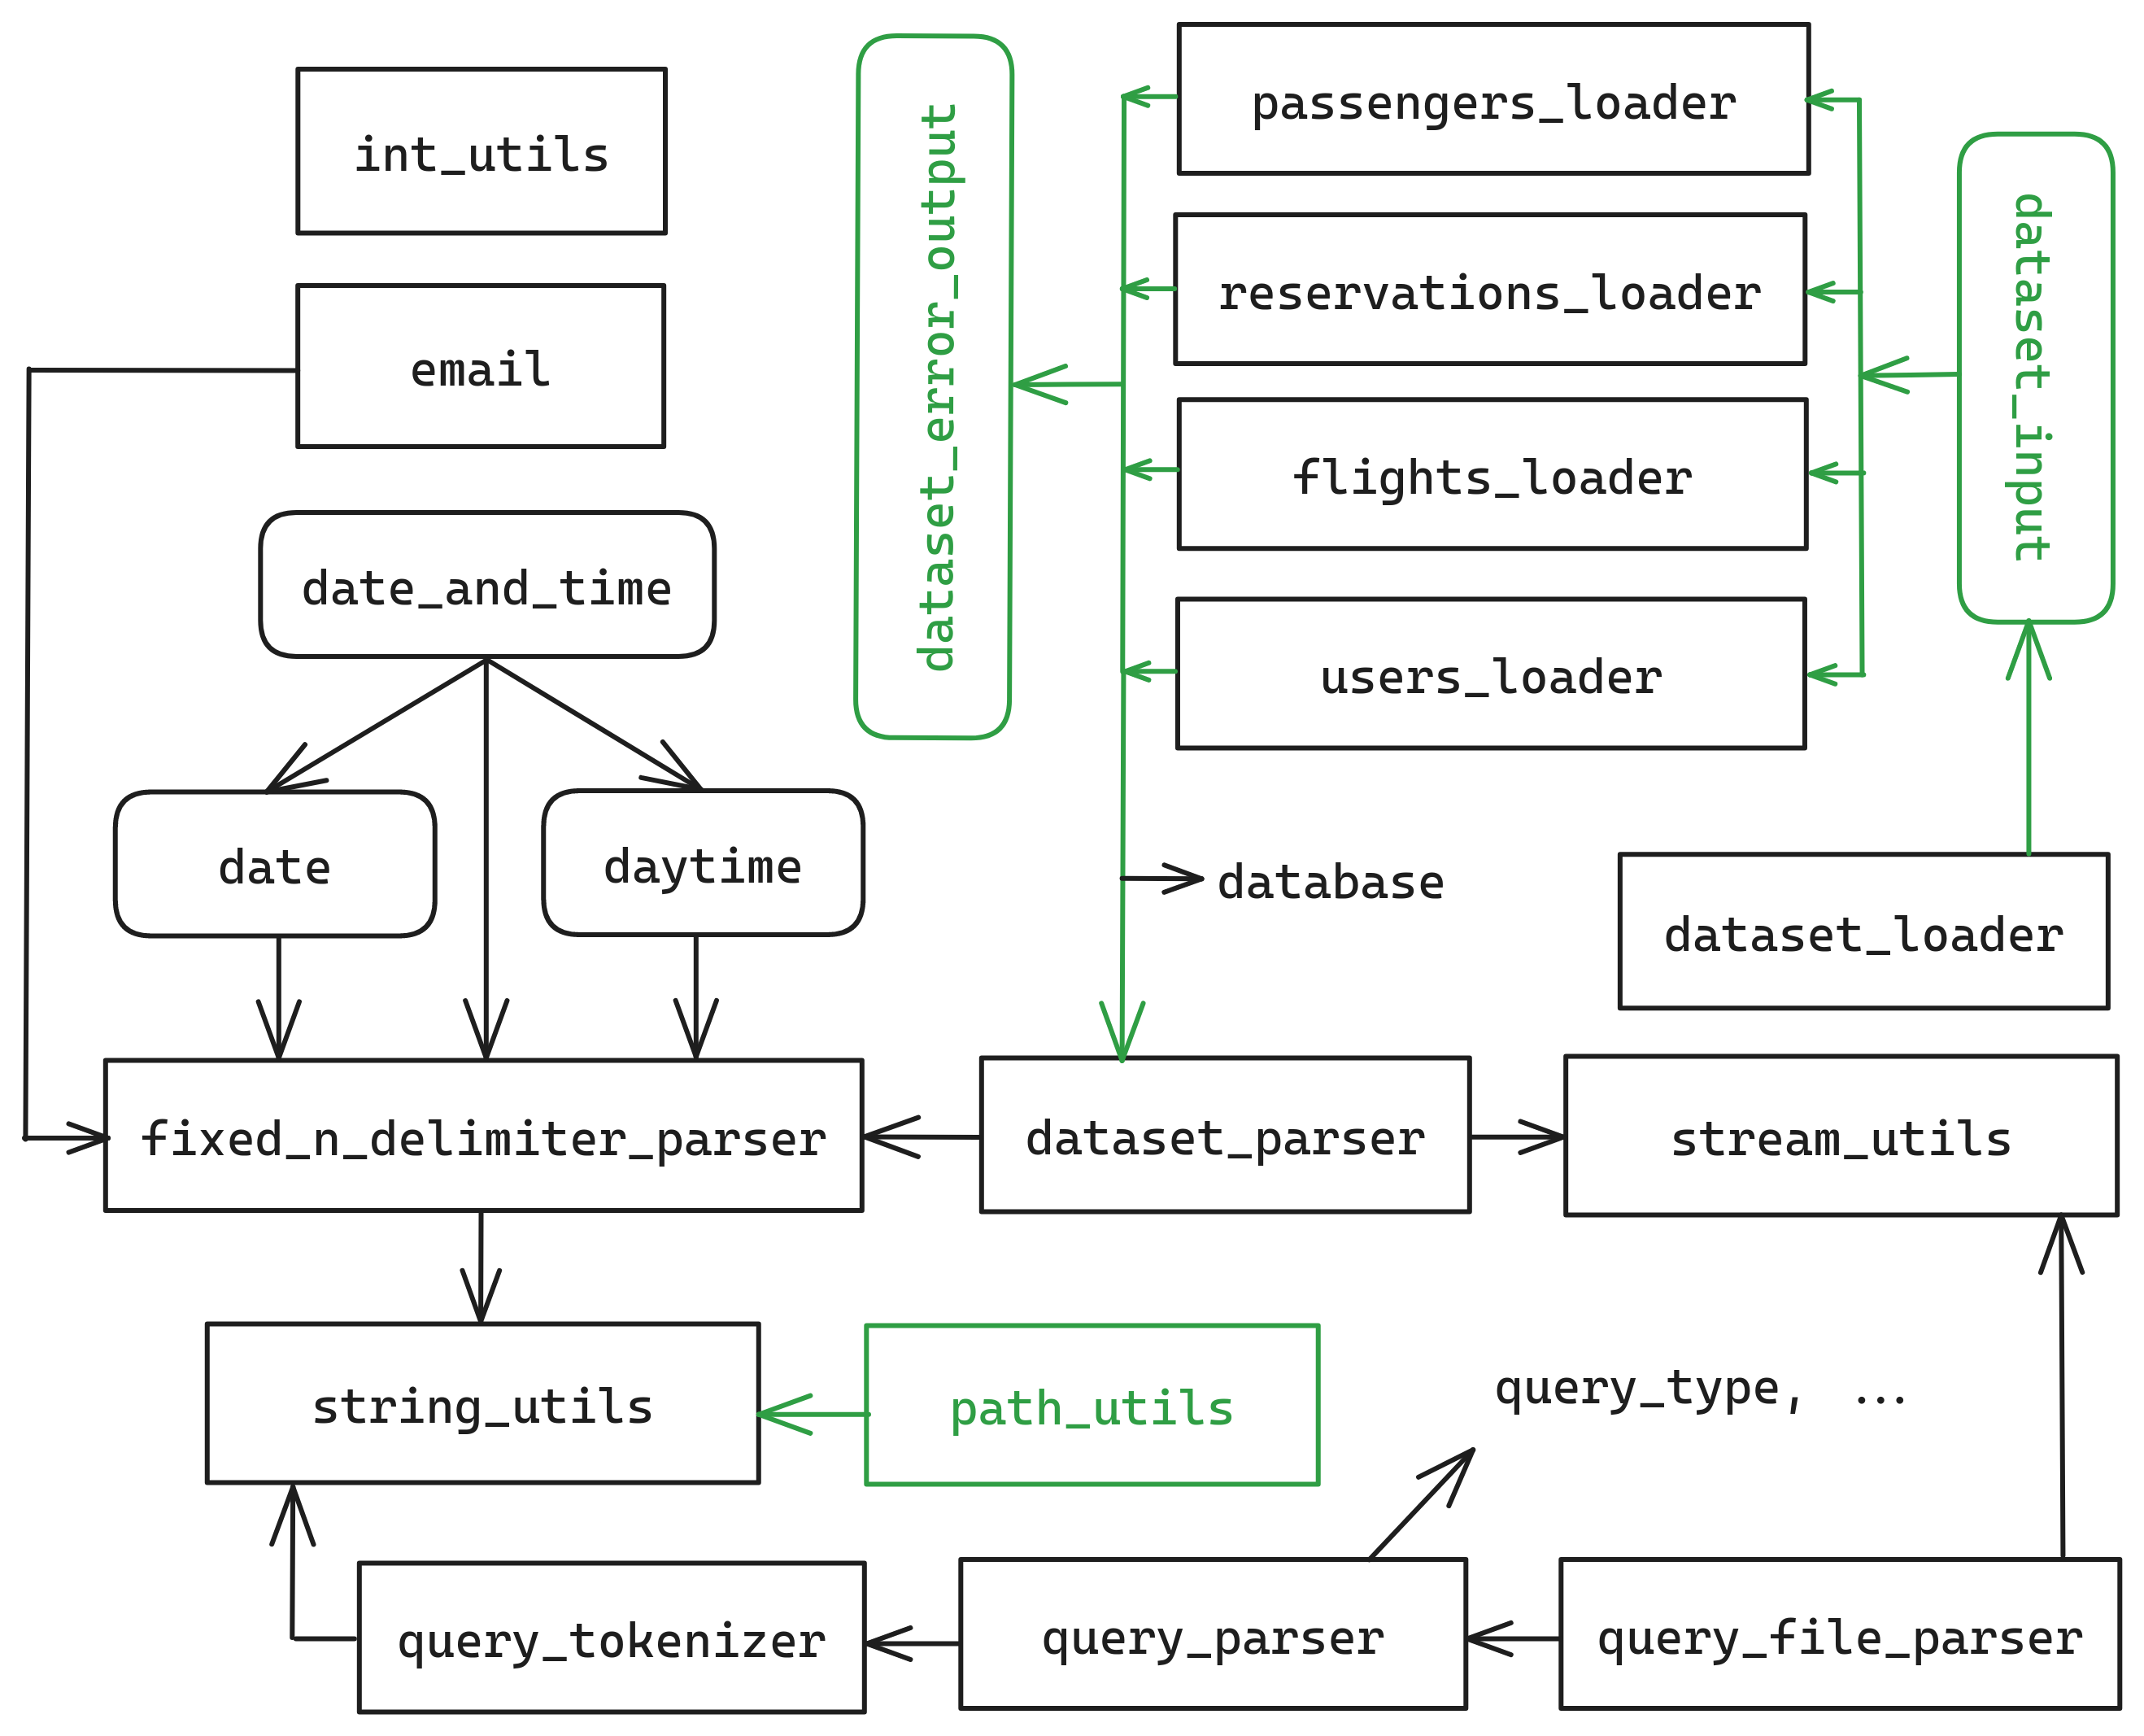
\includegraphics[scale=0.16]{res-fase2/parsing.png}
    \caption{Diagrama de dependências do subsistema de \emph{parsing}}
    \label{fig:parsing}
\end{figure}

Nesta fase do projeto, separámos em diferentes módulos as funcionalidades de \emph{input} de dados
e \emph{output} de erros num \emph{dataset}, antes concentradas no \texttt{dataset\_loader}. Agora,
este módulo apenas gere duas estruturas de dados formadas por \emph{handles} de ficheiros,
\texttt{dataset\_input} e \texttt{dataset\_error\_output}. Além disso, adicionámos o módulo
\texttt{path\_utils}, para manipulação de caminhos para ficheiros.

\subsection{Entidades}
\label{sec:entities}

\begin{figure}[H]
    \centering
    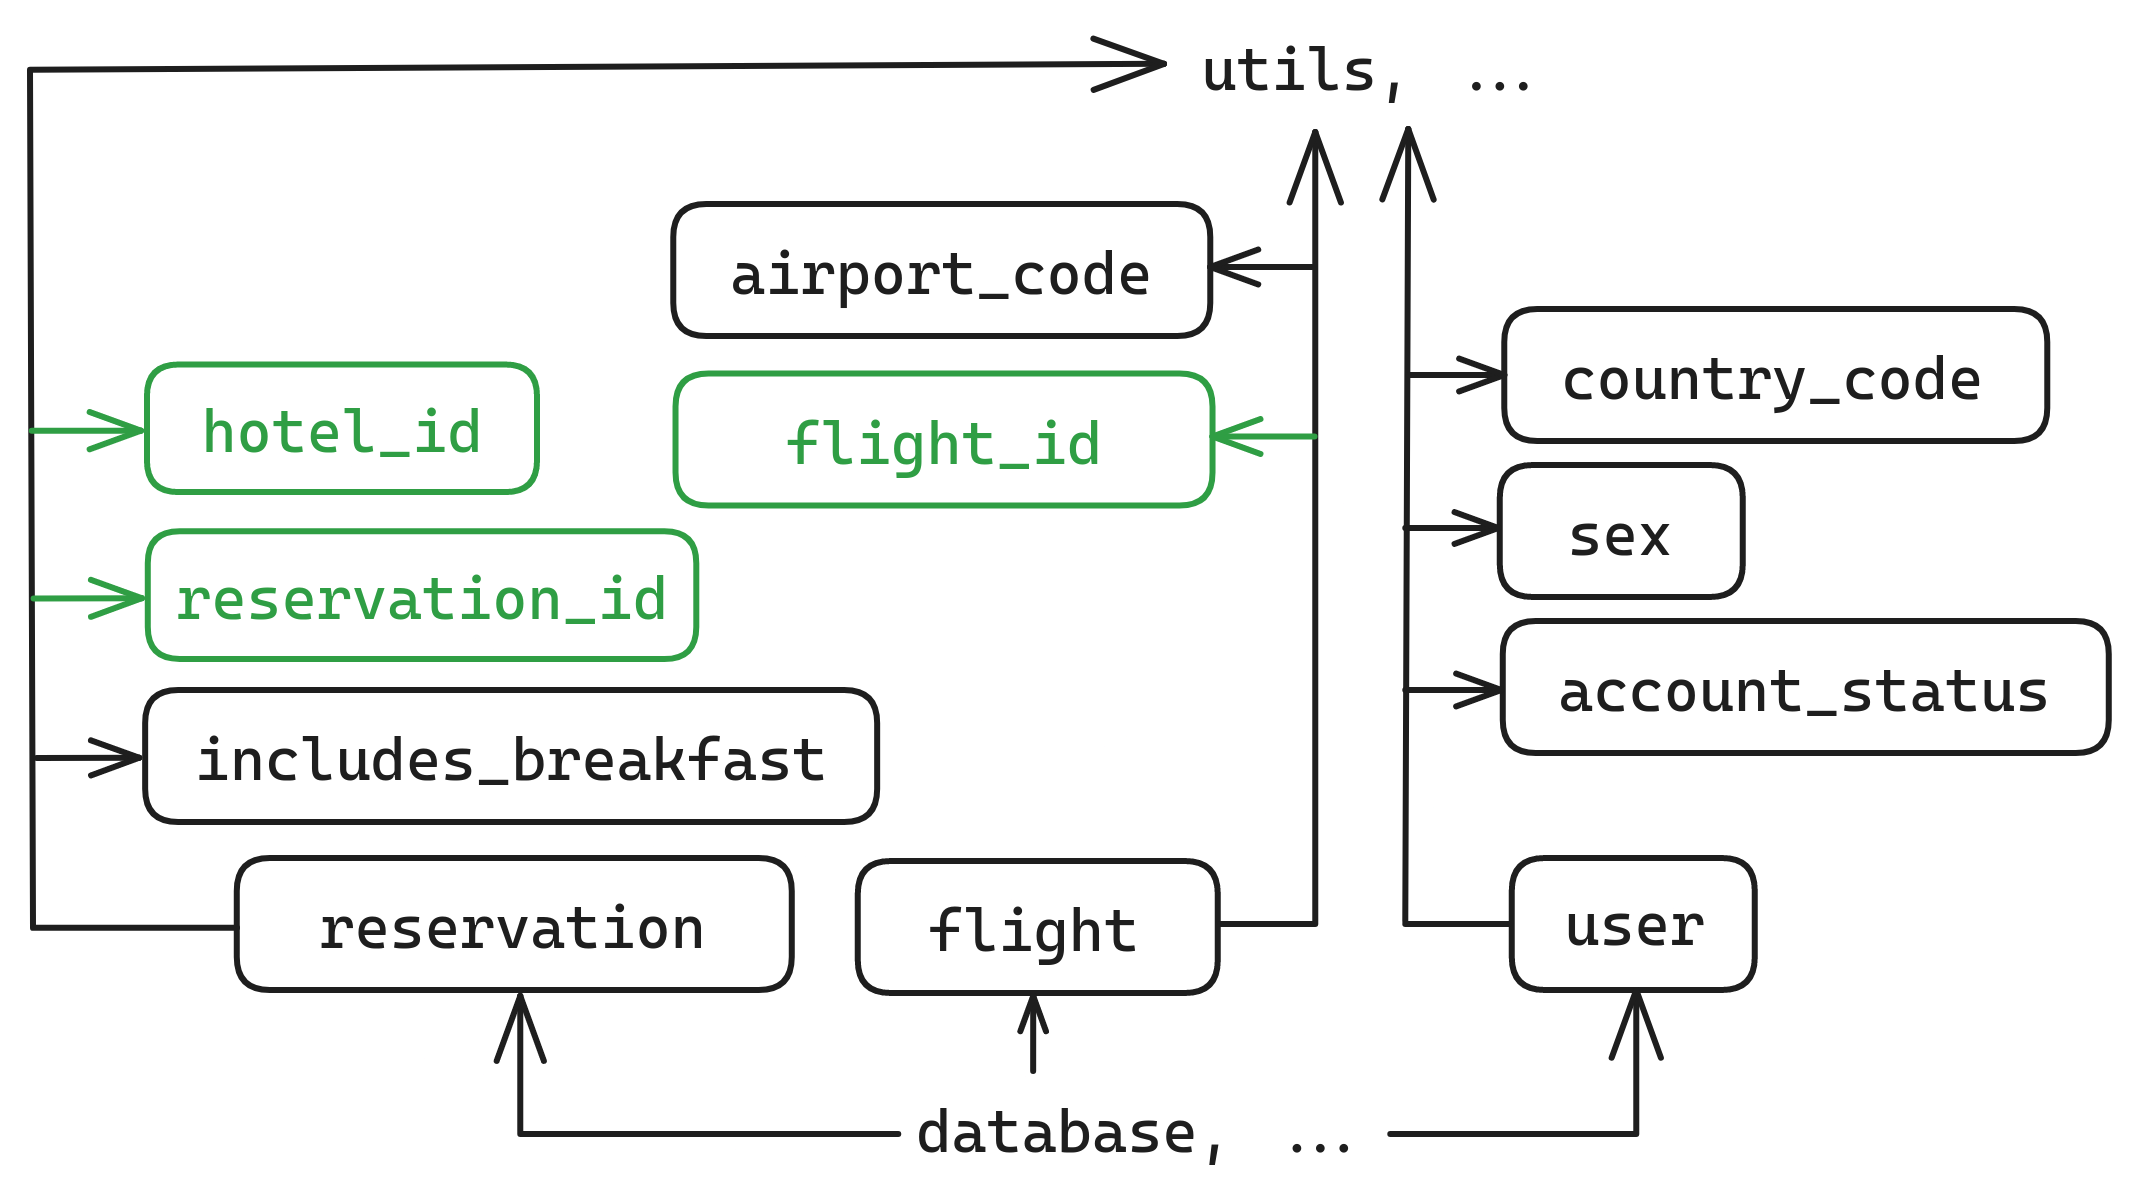
\includegraphics[scale=0.16]{res-fase2/entities.png}
    \caption{Diagrama de dependências das entidades da aplicação}
    \label{fig:entities}
\end{figure}

Nas entidades, criámos módulos para os identificadores de voos, reservas e hotéis, de modo a remover
código de \emph{parsing} e \emph{display} previamente duplicado em vários locais da \emph{codebase}.
Ademais, passaram a ser os \emph{setters} das entidades a validar se os valores providenciados para
os seus campos são válidos. Este antes era o trabalho dos módulos \texttt{*\_loader}, sendo possível
ao programador, usando \emph{setters}, criar uma entidade inválida.

\subsection{Catálogos}
\label{sec:catalogs}

\begin{figure}[ht]
    \centering
    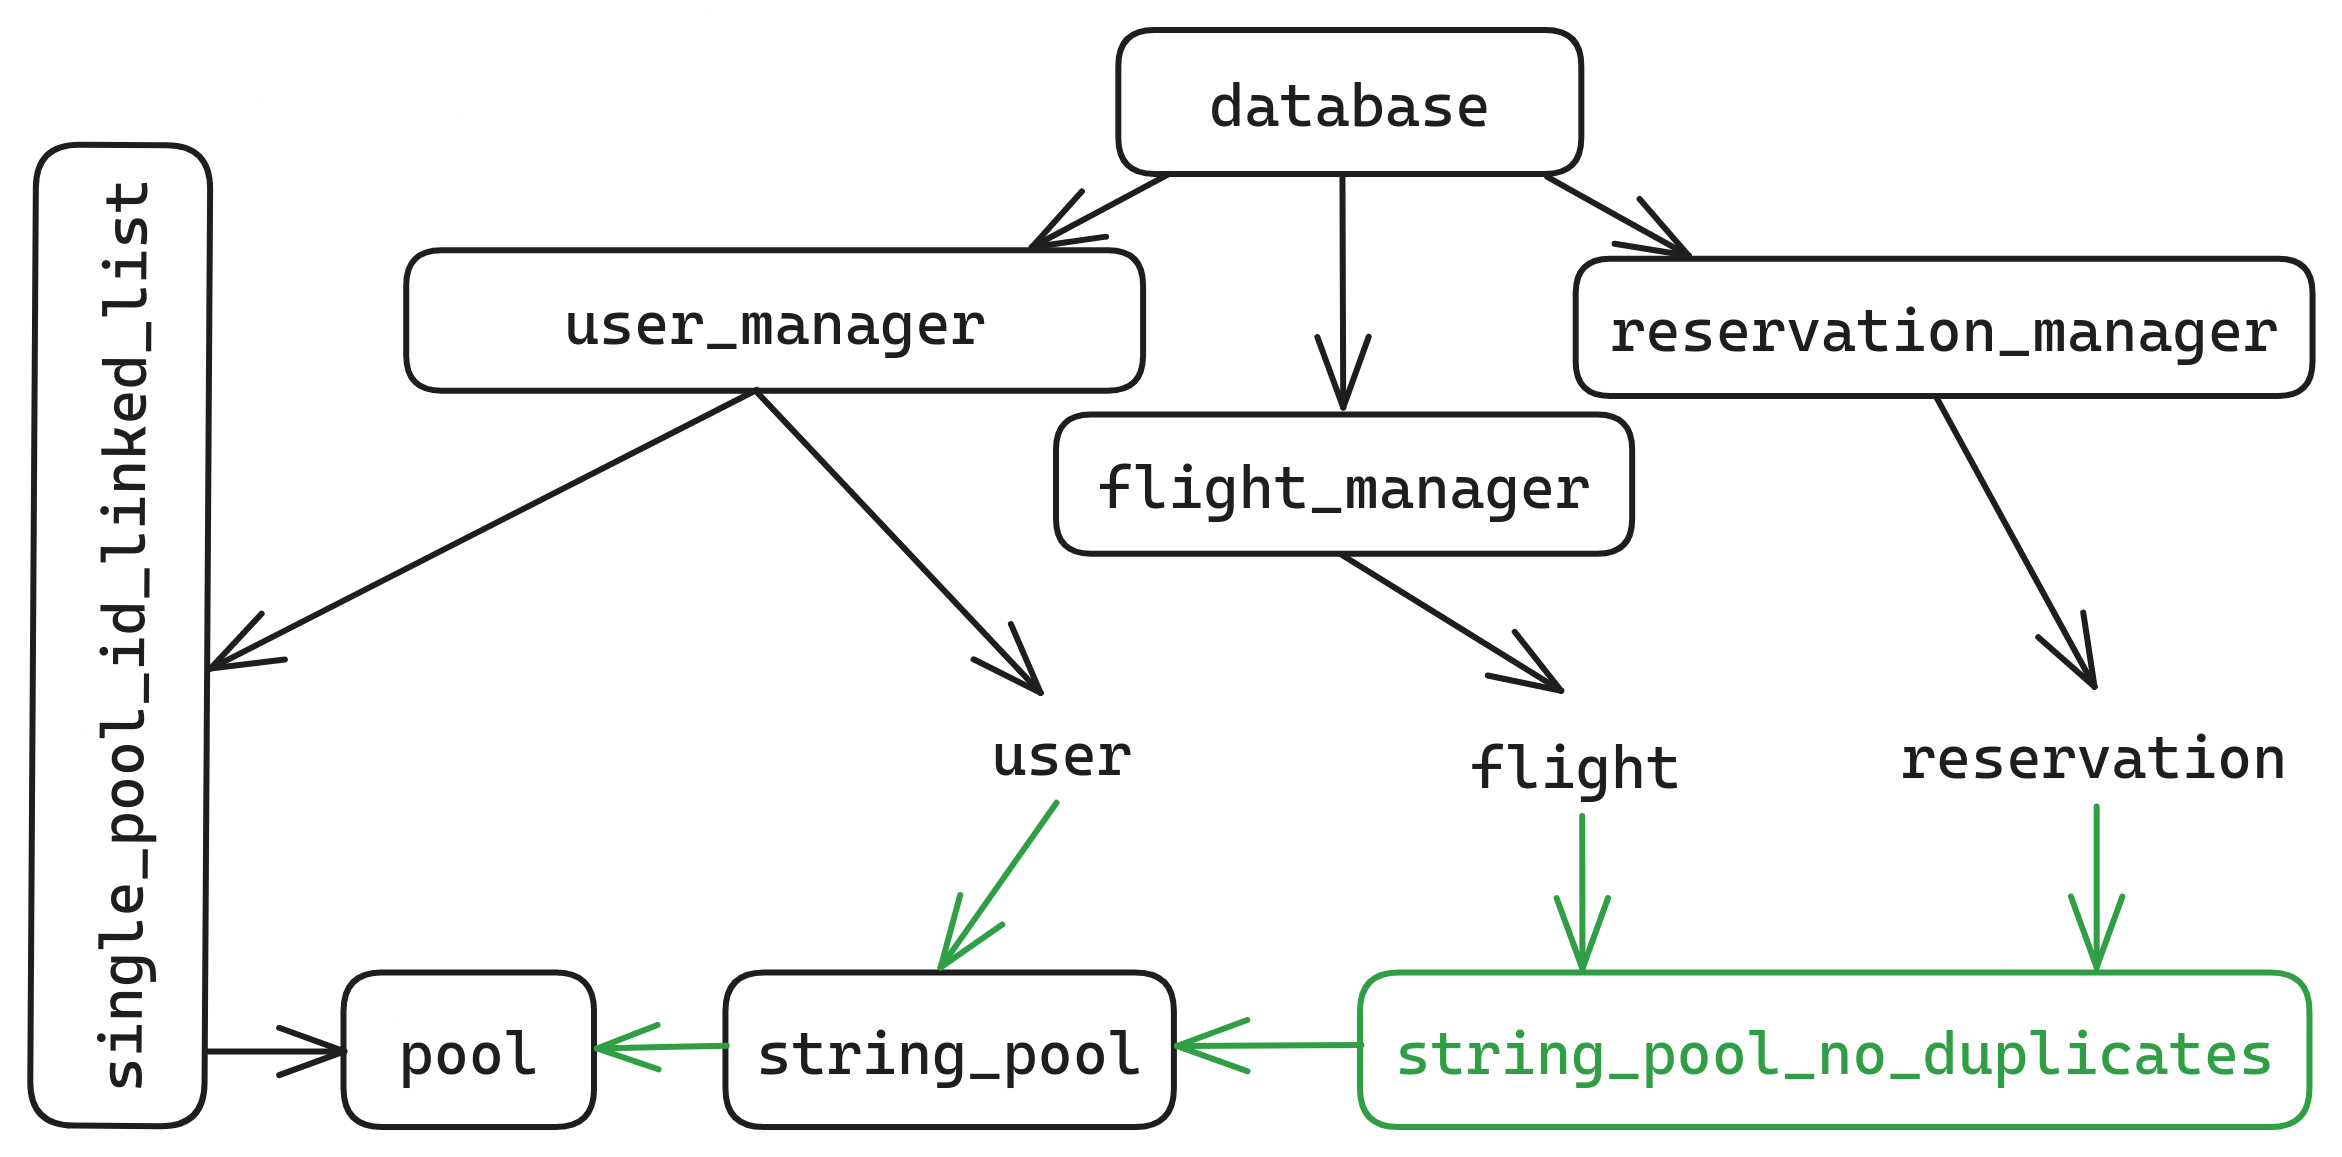
\includegraphics[scale=0.17]{res-fase2/database.png}
    \caption{Diagrama de dependências dos catálogos na aplicação}
    \label{fig:catalogs}
\end{figure}

De modo a diminuir o uso de memória da aplicação, criámos o \texttt{string\_pool\_no\_duplicates},
um novo alocador que armazena apenas uma vez \emph{strings} sujeitas a repetição, como nomes de
hotéis e de companhias aéreas.

Quanto às novas relações de dependência, removemos muito código duplicado ao adaptar a
\texttt{pool}, para com ela ser possível implementar a \texttt{string\_pool}. Por último, as
entidades passam a depender dos alocadores, por motivos explicados em
\nameref{sec:allocator-conciliation}.

\subsection{\emph{Queries}}
\label{sec:queries}

\begin{figure}[ht]
    \centering
    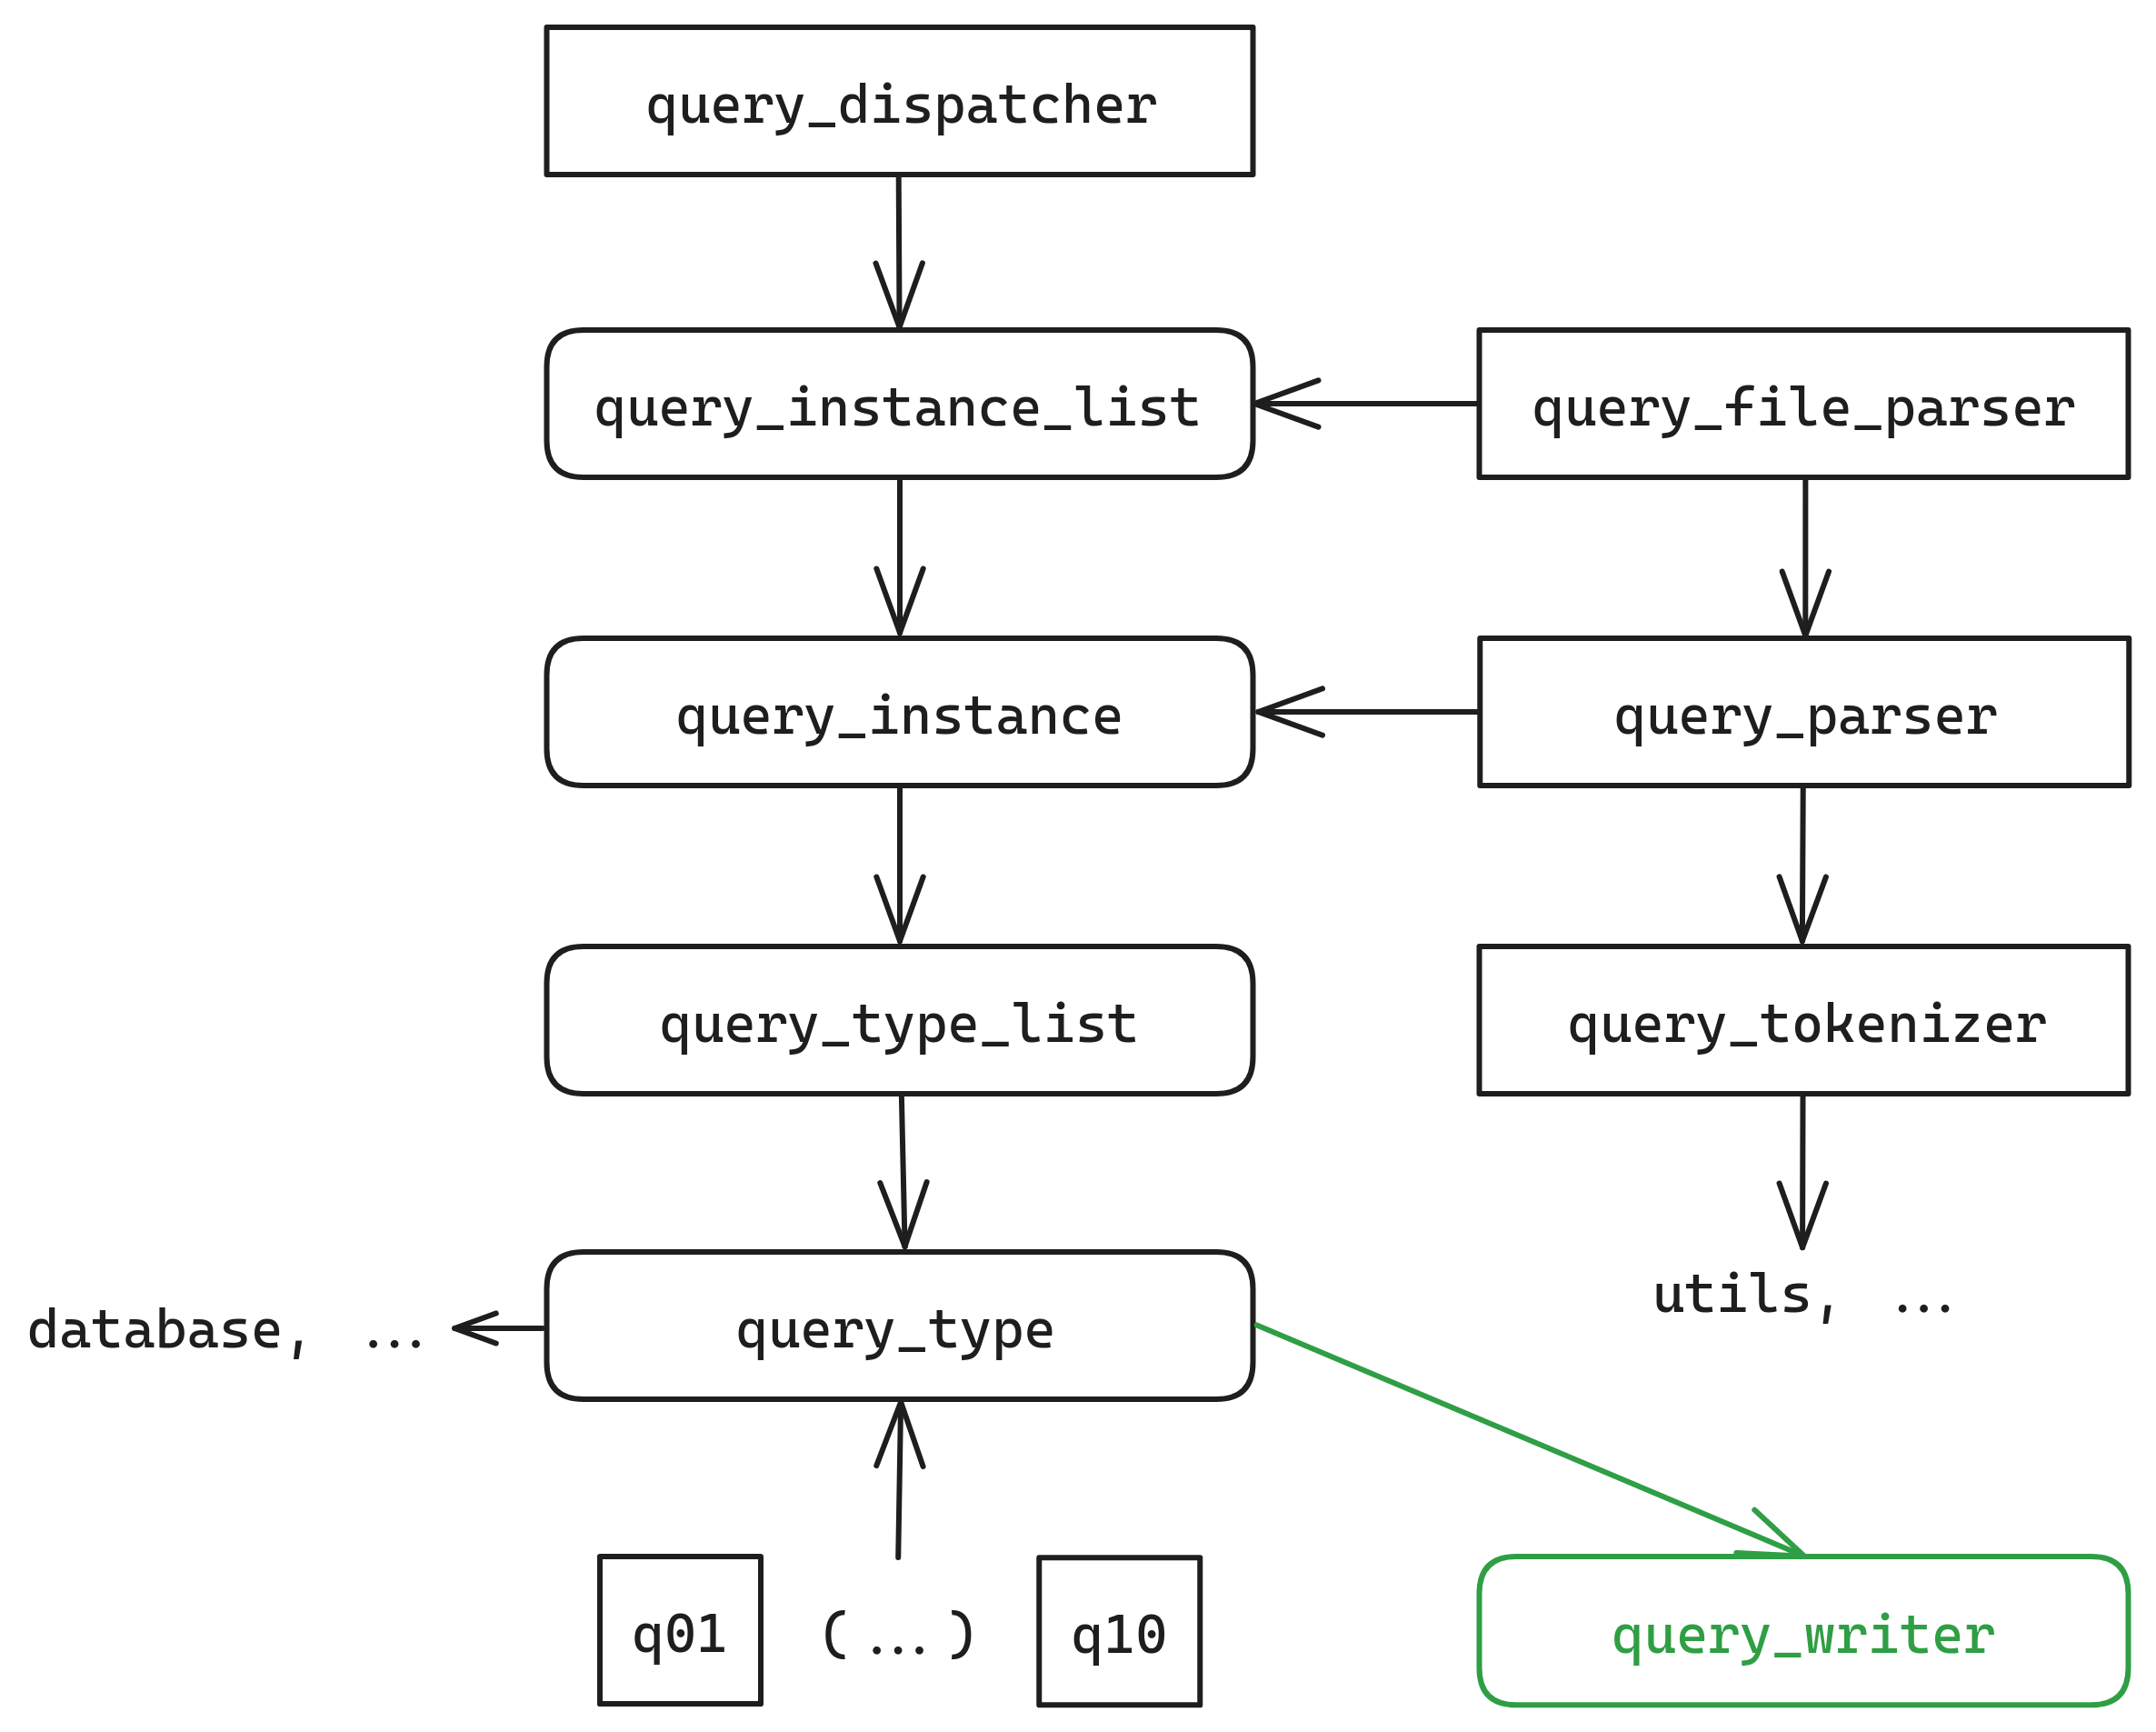
\includegraphics[scale=0.15]{res-fase2/queries.png}
    \caption{Diagrama de dependências do subsistema de \emph{queries}}
    \label{fig:queries}
\end{figure}

Como todas as \emph{queries} apresentam a mesma formatação de \emph{output}, adicionámos o
\texttt{query\_writer}, uma estrutura que formata o \emph{output} de uma \emph{query}
automaticamente, e o escreve para um ficheiro (modo \emph{batch}) ou para um conjunto de linhas em
memória (modo interativo). Os módulos \texttt{GConstPtrArray} e \texttt{GConstKeyHashTable} são
explicados em \nameref{sec:glib-conciliation}. Segue-se a descrição do funcionamento das
\emph{queries} novas e das que sofreram mudanças significativas:

\begin{itemize}
    \item \textbf{Q05} - Listagem dos voos com origem num dado aeroporto entre duas datas. Com uma
                         única iteração pelos voos para todas as \emph{queries} deste tipo,
                         verifica-se se cada voo cumpre as condições para ser parte da resposta
                         a uma \emph{query}. Em caso afirmativo, adiciona-se esse voo a um
                         \emph{array} associado à \emph{query}. A execução de cada \emph{query}
                         passa apenas pela ordenação e apresentação do seu \emph{array}
                         correspondente.

    \item \textbf{Q07} - Listagem dos aeroportos com maior mediana de atrasos. Com uma única
                         iteração pelos voos para todas as \emph{queries} deste tipo, gera-se uma
                         tabela de \emph{hash} que associa aeroportos a \emph{arrays} de atrasos.
                         Depois, calcula-se a mediana para cada \emph{array}, gerando-se outra
                         \emph{hash table}, entre aeroportos e medianas. Executar cada \emph{query}
                         consiste na consulta direta desta tabela.

    \item \textbf{Q08} - Cálculo da receita de um hotel entre duas datas. Com uma única iteração
                         pelas reservas para todas as \emph{queries} deste tipo, gera-se uma tabela
                         de \emph{hash} que associa \emph{queries} a receitas. Interseta-se, para
                         cada reserva, o intervalo de noites dormidas com o intervalo pedido em cada
                         \emph{query}, para o cálculo do número de noites e da receita total.
                         Executar cada \emph{query} consiste simplesmente na consulta da tabela
                         gerada.

    \item \textbf{Q09} - Listagem de todos os utilizadores cujo nome comece com um dado prefixo. A
                         nova implementação desta \emph{query} é muito semelhante à da \textbf{Q05},
                         mas iterando pelos utilizadores em vez dos voos. Esta solução é
                         significativamente mais veloz que a anterior, que fazia uma iteração pelos
                         utilizadores por \emph{query}.

    \item \textbf{Q10} - Cálculo de várias métricas gerais da aplicação. Com uma única iteração pela
                         totalidade dos catálogos para todas as \emph{queries} deste tipo,
                         verifica-se se cada entidade deve ou não ser contada para a resposta a cada
                         \emph{query}. Como o acesso aos passageiros é feito utilizador a
                         utilizador, torna-se possível, usando uma \emph{bitmask}, facilmente
                         discernir os passageiros únicos. A execução de cada \emph{query} torna-se
                         uma simples pesquisa pelas respostas previamente geradas.
\end{itemize}

\subsection{Modo interativo}
\label{sec:interactive-mode}

\begin{figure}[H]
    \centering
    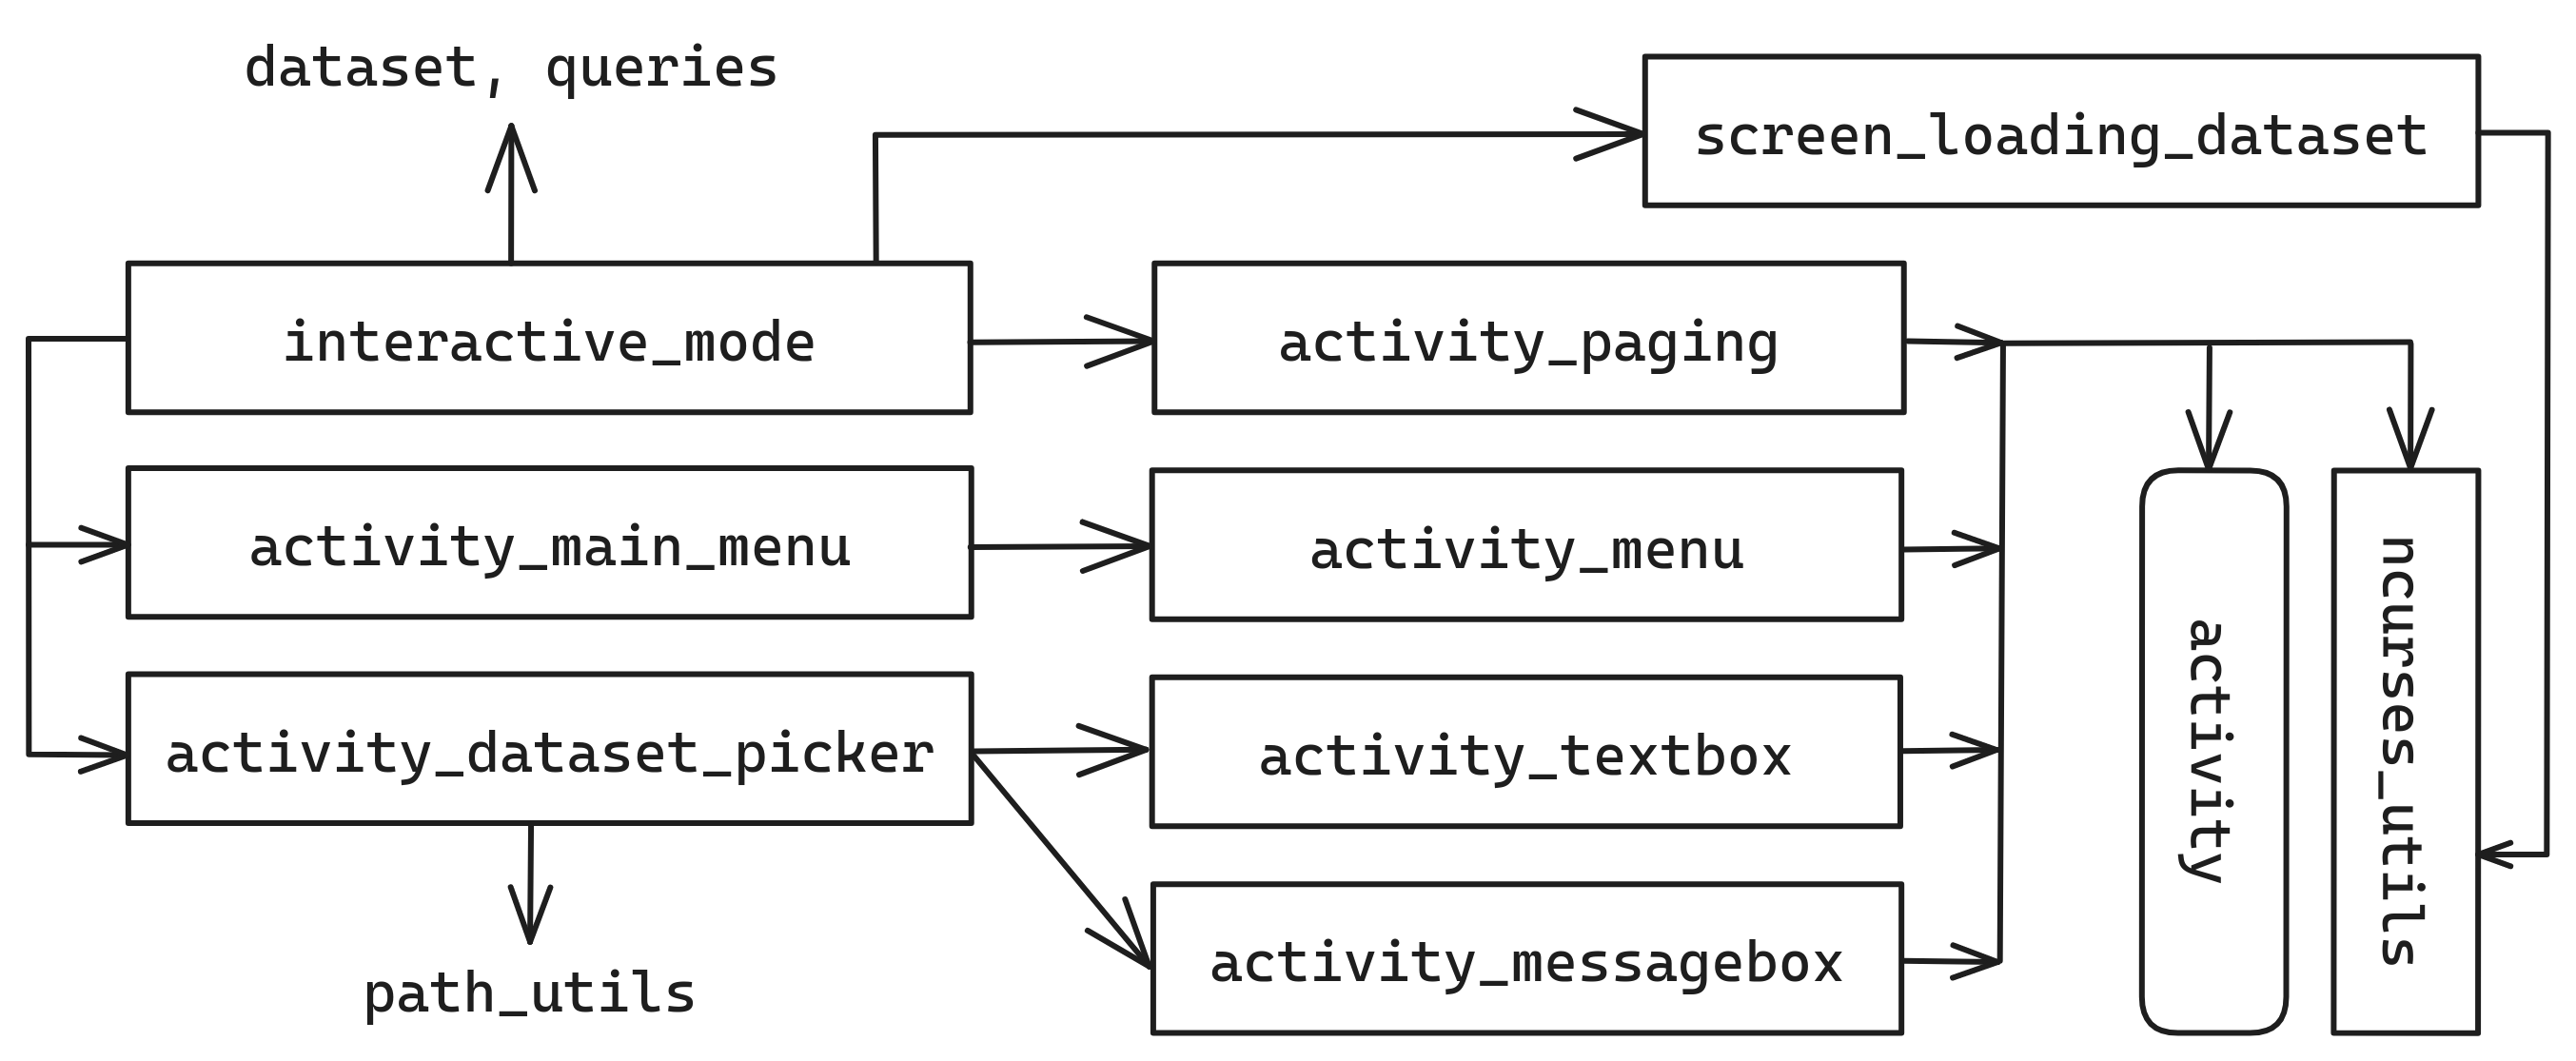
\includegraphics[scale=0.16]{res-fase2/interactive.png}
    \caption{Diagrama de dependências do modo interativo}
    \label{fig:interactive}
\end{figure}

O modo interativo revolve à volta do conceito de atividade (\texttt{activity}), uma estrutura
polimórfica que gere o \emph{loop} de eventos de uma interface \texttt{curses}. Imagens das
atividades implementadas podem ser encontradas em \nameref{sec:interactive-screenshots}.
\texttt{screen\_loading\_dataset} não responde a eventos, mas desenha no ecrã que a aplicação se
encontra a ler um \emph{dataset}. O módulo \texttt{interactive\_mode} é responsável por controlar a
troca entre atividades, formando a aplicação final. Neste subsistema, destaca-se a facilidade de
uso (instruções em todas as interfaces, explorador de ficheiros para escolher um \emph{dataset},
\dots) e o suporte para Unicode no \emph{layout} das atividades.

\subsection{Subsistema de testes}
\label{sec:testing-subsystem}

\begin{figure}[ht]
    \centering
    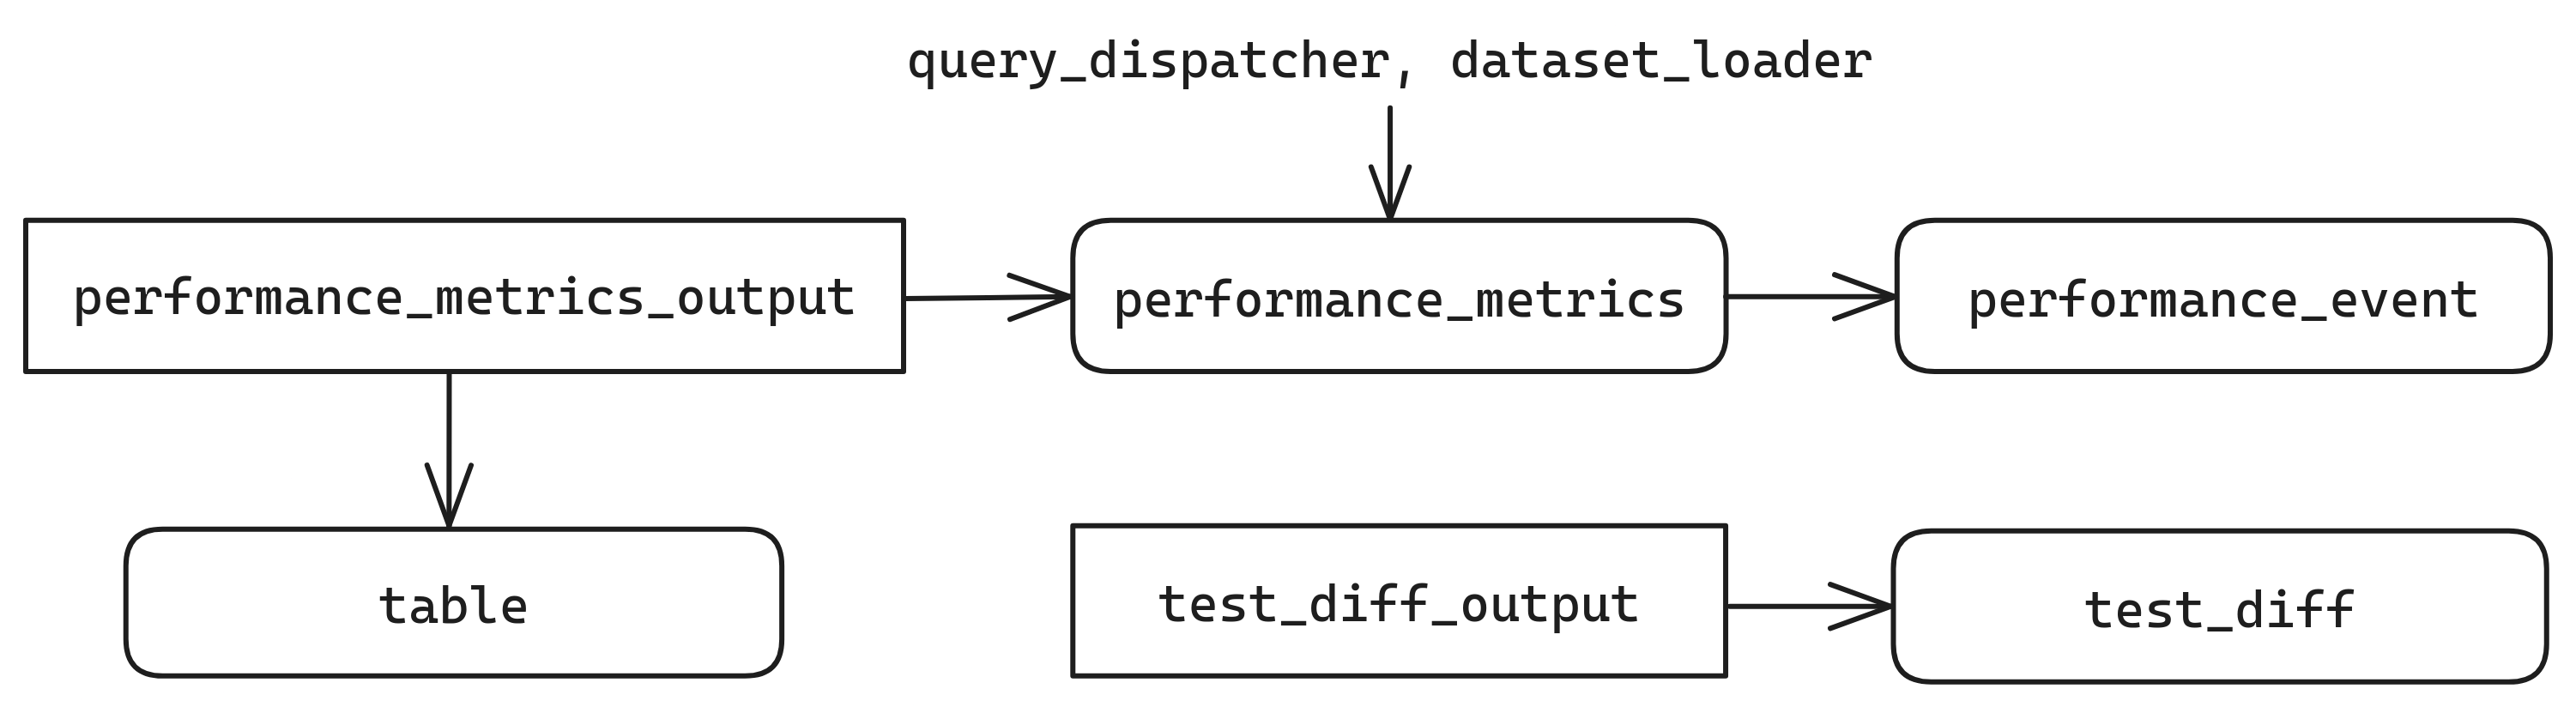
\includegraphics[scale=0.15]{res-fase2/testing.png}
    \caption{Diagrama de dependências do subsistema de testes}
    \label{fig:testing}
\end{figure}

Os testes de desempenho baseiam-se num \texttt{performance\_event}, uma medição do tempo e da
diferença do uso de memória entre dois instantes. \texttt{performance\_metrics} são um conjunto de
eventos de desempenho, produzidos ao longo do decorrer da aplicação, e mostrados ao utilizador no
final da sua execução (\texttt{performance\_metrics\_output}). Este módulo apresenta várias tabelas
(\texttt{table}), relativas ao uso de recursos computacionais na leitura de cada parte do
\emph{dataset} e na execução de cada \emph{query}.

Os testes funcionais são implementados por \texttt{test\_diff}, que calcula as diferenças entre
duas diretorias (resultados esperados \emph{vs} obtidos), que são depois apresentadas ao utilizador
por \texttt{test\_diff\_output}. Imagens dos resultados de ambos os tipos de teste encontram-se
em \nameref{sec:testing-screenshots}.

\section{Modularidade e encapsulamento}
\label{sec:modularity-and-encapsulation}

\subsection{Modularidade}
\label{sec:modularity}

Nesta fase, no âmbito da modularidade, procurámos separar os módulos de I/O e reduzir a duplicação
de código relativa aos identificadores das entidades. Ademais, escrevemos um \emph{script} que
automaticamente gera um grafo de dependências com todos os módulos. Este permitiu-nos corrigir erros
nos diagramas nos relatórios, e encontrar dependências circulares, que prontamente resolvemos.

\begin{figure}[ht]
    \centering
    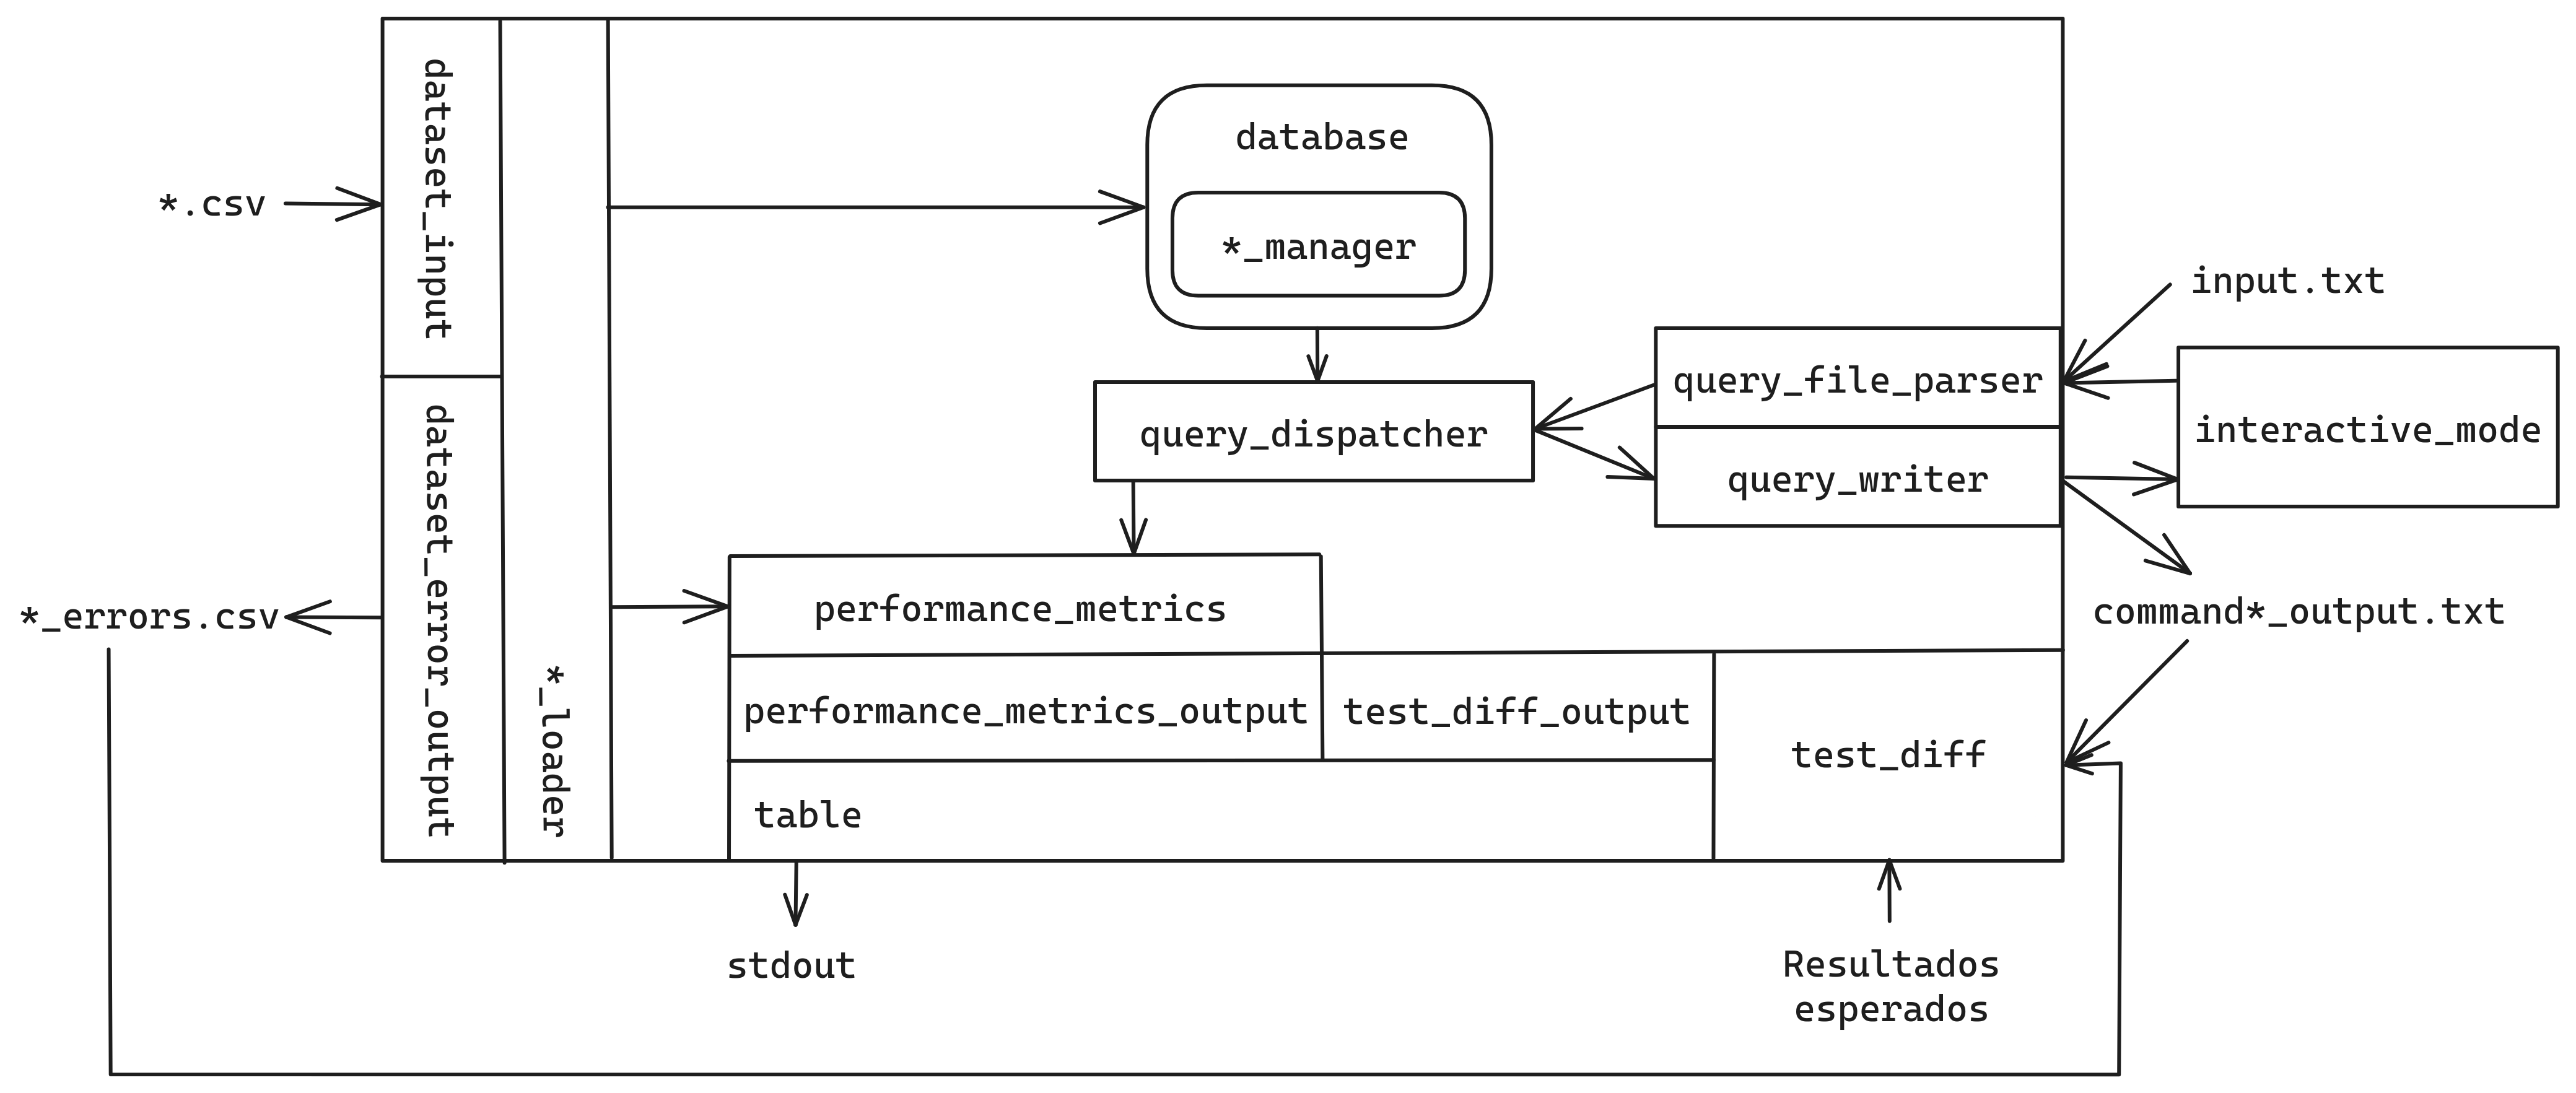
\includegraphics[scale=0.115]{res-fase2/io.png}
    \caption{Transferência e armazenamento de dados pelos \textbf{principais} módulos da aplicação.
             Observam-se os novos módulos de I/O.}
    \label{fig:io}
\end{figure}

\begin{figure}[ht]
    \centering
    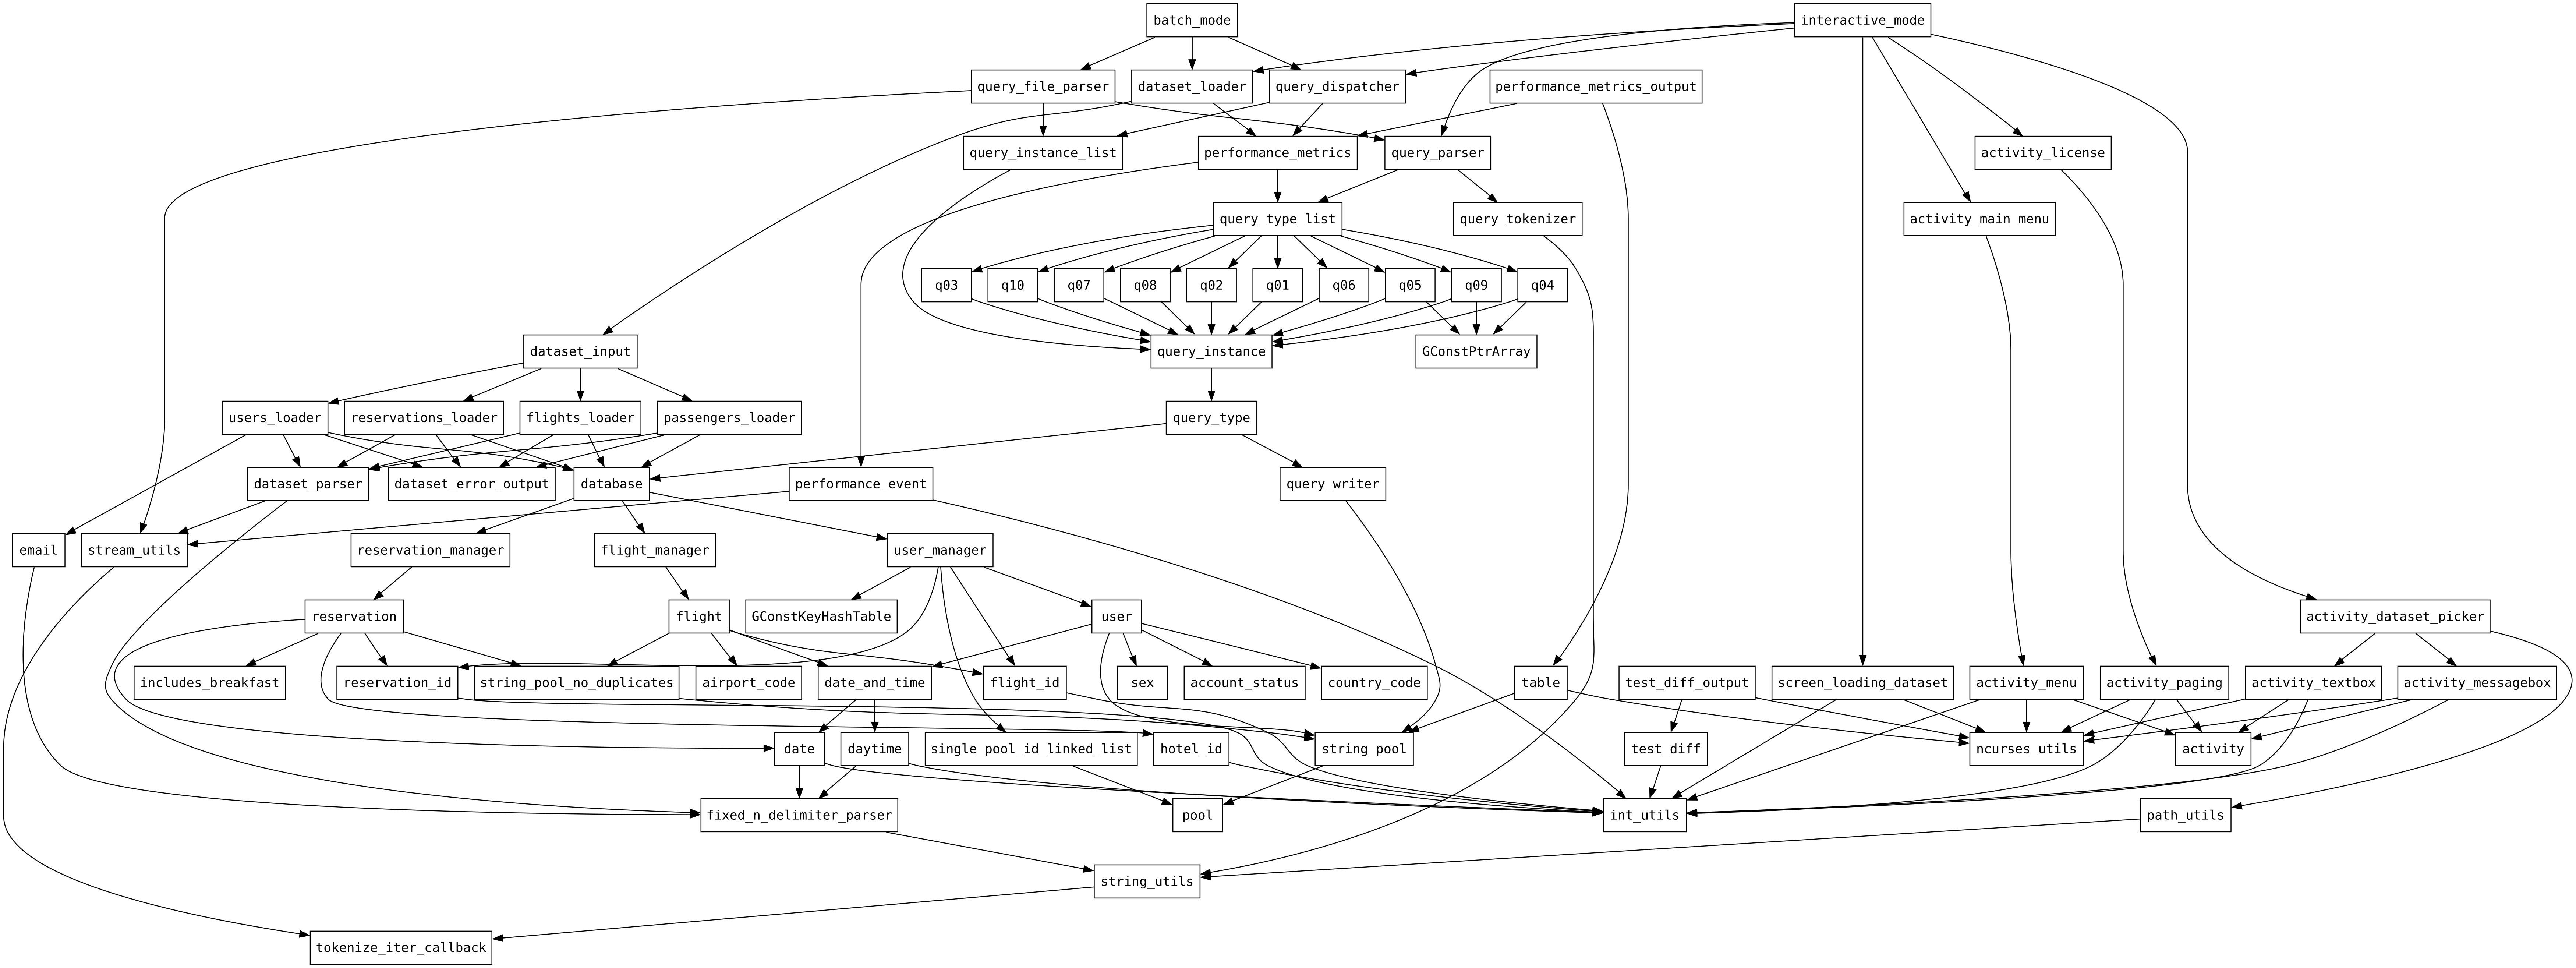
\includegraphics[scale=0.09]{res-fase2/global_dependencies.png}
    \caption{Grafo de dependências de toda a aplicação. Foi gerado automaticamente e não há
             distinção entre tipos de módulos.}
    \label{fig:global-dependencies}
\end{figure}

\subsection{Encapsulamento}
\label{sec:encapsulation}

\subsubsection{\emph{The great refactoring}}
\label{sec:the-great-refactoring}

Apesar de, na primeira fase deste trabalho, termos definido \emph{getters} e \emph{setters} para as
estruturas de dados, estávamos cientes da ausência de encapsulamento, pois vários \emph{getters}
devolviam apontadores mutáveis para dados no interior das estruturas. Como nunca escrevíamos para
estes apontadores, torná-los constantes provou-se a melhor solução para o encapsulamento.

Este processo de aplicar a \emph{keyword} \texttt{const} aos argumentos dos métodos e aos seus
valores devolvidos provou-se moroso: a cada \texttt{const} adicionado, vários módulos deixavam de
compilar devido a erros de tipos, causando uma reação em cadeia de mudanças necessárias. No processo
de encapsulamento, adicionámos também métodos de cópia profunda (semelhantes aos \emph{copy
constructors} de C++) à maioria das estruturas de dados da aplicação. \footnote{Com exceção de
alocadores (\emph{pools}) e estruturas que contêm \texttt{FILE *}.}

Apercebemo-nos da importância de uma interface modular bem pensada que dispensa mudanças, já que
estas se provaram muito trabalhosas. No modo interativo e no subsistema de testes, como pensámos nas
interfaces dos módulos com encapsulamento em mente, não precisámos de gastar tempo na sua correção.

\subsubsection{Conciliação com alocadores}
\label{sec:allocator-conciliation}

As únicas estruturas de dados que expõem memória do seu interior são os alocadores \texttt{pool} e
\texttt{string\_pool}. Não encaramos isto como um problema para o encapsulamento, pois é algo que
qualquer alocador tem de fazer (por exemplo, o método \texttt{malloc} expõe memória da arena com
que é implementado).

Previamente, durante uma inserção na base de dados, as entidades e os seus campos eram alocados
pelos \emph{managers} nas \emph{pools}, e não pelas entidades em si. Resolvemos este problema usando
uma estratégia semelhante à utilizada na linguagem Zig: se um método precisa de alocar memória,
então leva um alocador como argumento:

\begin{center}
    \texttt{fn validate(allocator: Allocator, s: []const u8) Allocator.Error!bool}
\end{center}

Este método de Zig valida texto JSON, levando também como argumento um alocador. Na nossa aplicação
C, é dada a possibilidade de se usar uma \emph{pool}, ou de se passar o valor \texttt{NULL} ao
argumento do alocador, para o uso de \texttt{malloc}:

\bgroup
    \setlength\tabcolsep{0.5mm}
    \begin{center}
        \begin{tabular}{rll}
            \texttt{user\_t *user\_clone\char"0028} & \texttt{pool\_t} & \texttt{*allocator,} \\
            & \texttt{string\_pool\_t} \hspace{1mm} & \texttt{*string\_allocator,} \\
            & \texttt{const user\_t} & \texttt{*user\char"0029;}
        \end{tabular}
    \end{center}
\egroup

\subsubsection{Conciliação com a \texttt{glib}}
\label{sec:glib-conciliation}

O uso de \texttt{const} trata-se de um contrato de que um método não irá modificar um objeto. A
documentação das estruturas genéricas da \texttt{glib} assegura isto.\footnote{Há algumas exceções
(como uma função \texttt{GDestroyNotify} ser providenciada), mas garantimos que a nossa solução para
este problema não permite nenhuma destas.} No entanto, estas utilizam \texttt{void *} sem o
\emph{qualifier} \texttt{const}, dado que os programadores podem querer usá-las para armazenar dados
mutáveis. A documentação da \texttt{glib} incentiva os programadores a usarem apontadores constantes
nas suas estruturas, desde que usem o tipo correto quando os reivindiquem.

No entanto, isto é altamente suscetível a erros, pelo que criámos \emph{wrappers} das estruturas da
\texttt{glib} para apontadores constantes, que lhes retiram o \emph{qualifier} nas inserções, e o
reinserem nas consultas. Isto reduz o potencial de erro do programa todo para pequenos métodos
facilmente validáveis, de um modo semelhante a conceito de \texttt{unsafe} em Rust.

\section{Desempenho}
\label{sec:performance}

\subsection{Melhorias}
\label{sec:performance-improvements}

Quando os \emph{datasets} de maior dimensão foram adicionados à plataforma de testes, já a nossa
aplicação apresentava um desempenho excelente. Mesmo assim, procurámos continuar a otimizar o nosso
programa.

Para reduzir ainda mais o uso de memória, introduzimos a \texttt{string\_pool\_no\_duplicates}, que
evita armazenar \emph{strings} repetidas. Ademais, reordenamos os campos nas estruturas de dados das
entidades, de modo a reduzir o \emph{padding} e o número de \emph{bytes} ocupados por cada uma.

A maioria do tempo de execução é gasto no \emph{parsing} do \emph{dataset}, onde apenas conseguimos
alcançar micro-otimizações nos métodos mais chamados (\texttt{strsep} e
\texttt{int\_utils\_parse\_positive}), determinados com recurso ao \texttt{callgrind}. As
\emph{queries} são praticamente instantâneas para um utilizador do modo interativo, e responsáveis
por apenas uma pequena fração do tempo de execução da aplicação. Logo, procurámos simplificar
as suas implementações, em vez de nos focarmos no seu desempenho.

\hspace{1cm}\parbox{15cm}{\small
    The real problem is that programmers have spent far too much time worrying about efficiency in
    the wrong places and at the wrong times; premature optimization is the root of all evil (or at
    least most of it) in programming.

    \begin{flushright}
        Knuth, D. E. (1974). Computer programming as an art. \\
        \emph{Association for Computing Machinery (ACM), 17}(12), 671. \\
        \url{https://doi.org/10.1145/361604.361612}
    \end{flushright}
}

Várias vezes se verificou um melhor desempenho utilizando estruturas de dados mais simples, com pior
complexidade assintótica, mas melhor localidade de memória. Foi importante garantir que os
catálogos, onde o número de entidades é muito elevado, usavam as estruturas com melhor comportamento
assintótico, mas tal não se provou tão relevante para dados auxiliares durante a execução das
\emph{queries}.

\subsection{\emph{Benchmarking}}
\label{sec:benchmarking}

Para testar o desempenho do programa, utilizámos a versão mais recente da aplicação nos seguintes
sistemas:

\begin{adjustwidth}{-1.5cm}{-1.5cm}
    \begin{center}
        \begin{tabular}{|l|c|c|c|c|}
            \hline
            & Desktop & Laptop & Mac & Tablet \\
            \hline
            CPU & Intel i3-7100 & Ryzen 7 5800H & Apple M1 Pro & Mediatek Helio P22T \\
            \hline
            Frequência\footnote{Em sistemas heterogéneos, a frequência do \emph{cluster} de maior
                                desempenho, dado que o nosso programa apenas usa um núcleo.} &
            3.9 GHz & 4.4 GHz & 3.2 GHz & 2.3 GHz \\
            \hline
            Memória & DDR4 2400 MT/s & DDR4 3200 MT/s & LPDDR5 6400 MT/s & LPDDR4X 4266 MT/s \\
            \hline
            Linux & 6.6.11 (chroot) & 5.15.91 & 5.15.73 (VM) & 4.9.190 \\
            \hline
            Compilador & GCC 12.2.0 & GCC 9.4.0 & GCC 11.4.0 & Clang 17.0.6 \\
            \hline
        \end{tabular}
    \end{center}
\end{adjustwidth}

O número de variáveis entre sistemas é elevadíssimo, pelo que apenas estamos interessados em
procurar padrões no desempenho do nosso programa comuns a todos os computadores, e não faremos
comparações entre eles.

A aplicação foi executada 10 vezes, com 500 \emph{queries} no \emph{dataset} grande com erros. As
execuções mais rápida e a mais lenta foram removidas. A partir das 8 restantes, calculam-se as
seguintes médias de tempo e uso de memória:

\begin{center}
    \begin{tabular}{|l|c|c|c|c|}
        \hline
        & Desktop & Laptop & Mac & Tablet \\
        \hline
        Utilizadores (s) & ? & ? & ? & ? \\
        \hline
        Voos (s) & ? & ? & ? & ? \\
        \hline
        Reservas (s) & ? & ? & ? & ? \\
        \hline
        Passageiros (s) & ? & ? & ? & ? \\
        \hline
        \emph{Queries} (s) & ? & ? & ? & ? \\
        \hline
        Tempo total (s) & ? & ? & ? & ? \\
        \hline
        Pico de memória (MiB) & ? & ? & ? & ? \\
        \hline
    \end{tabular}
\end{center}

% TODO - benchmarking

\subsection{Possíveis melhorias}
\label{sec:possible-performance-improvements}

Como mencionado acima, não vemos as \emph{queries} como um potencial local onde procurar
otimizações. A parte mais lenta do nosso programa é a leitura de um \emph{dataset}, onde já
otimizámos a localidade de memória e a complexidade algorítmica de inserção o mais que fomos
capazes. Sem sacrifício da modularidade e do encapsulamento, não vemos mais otimizações viáveis
que não a paralelização da leitura do \emph{dataset}:

\begin{figure}[h]
    \centering
    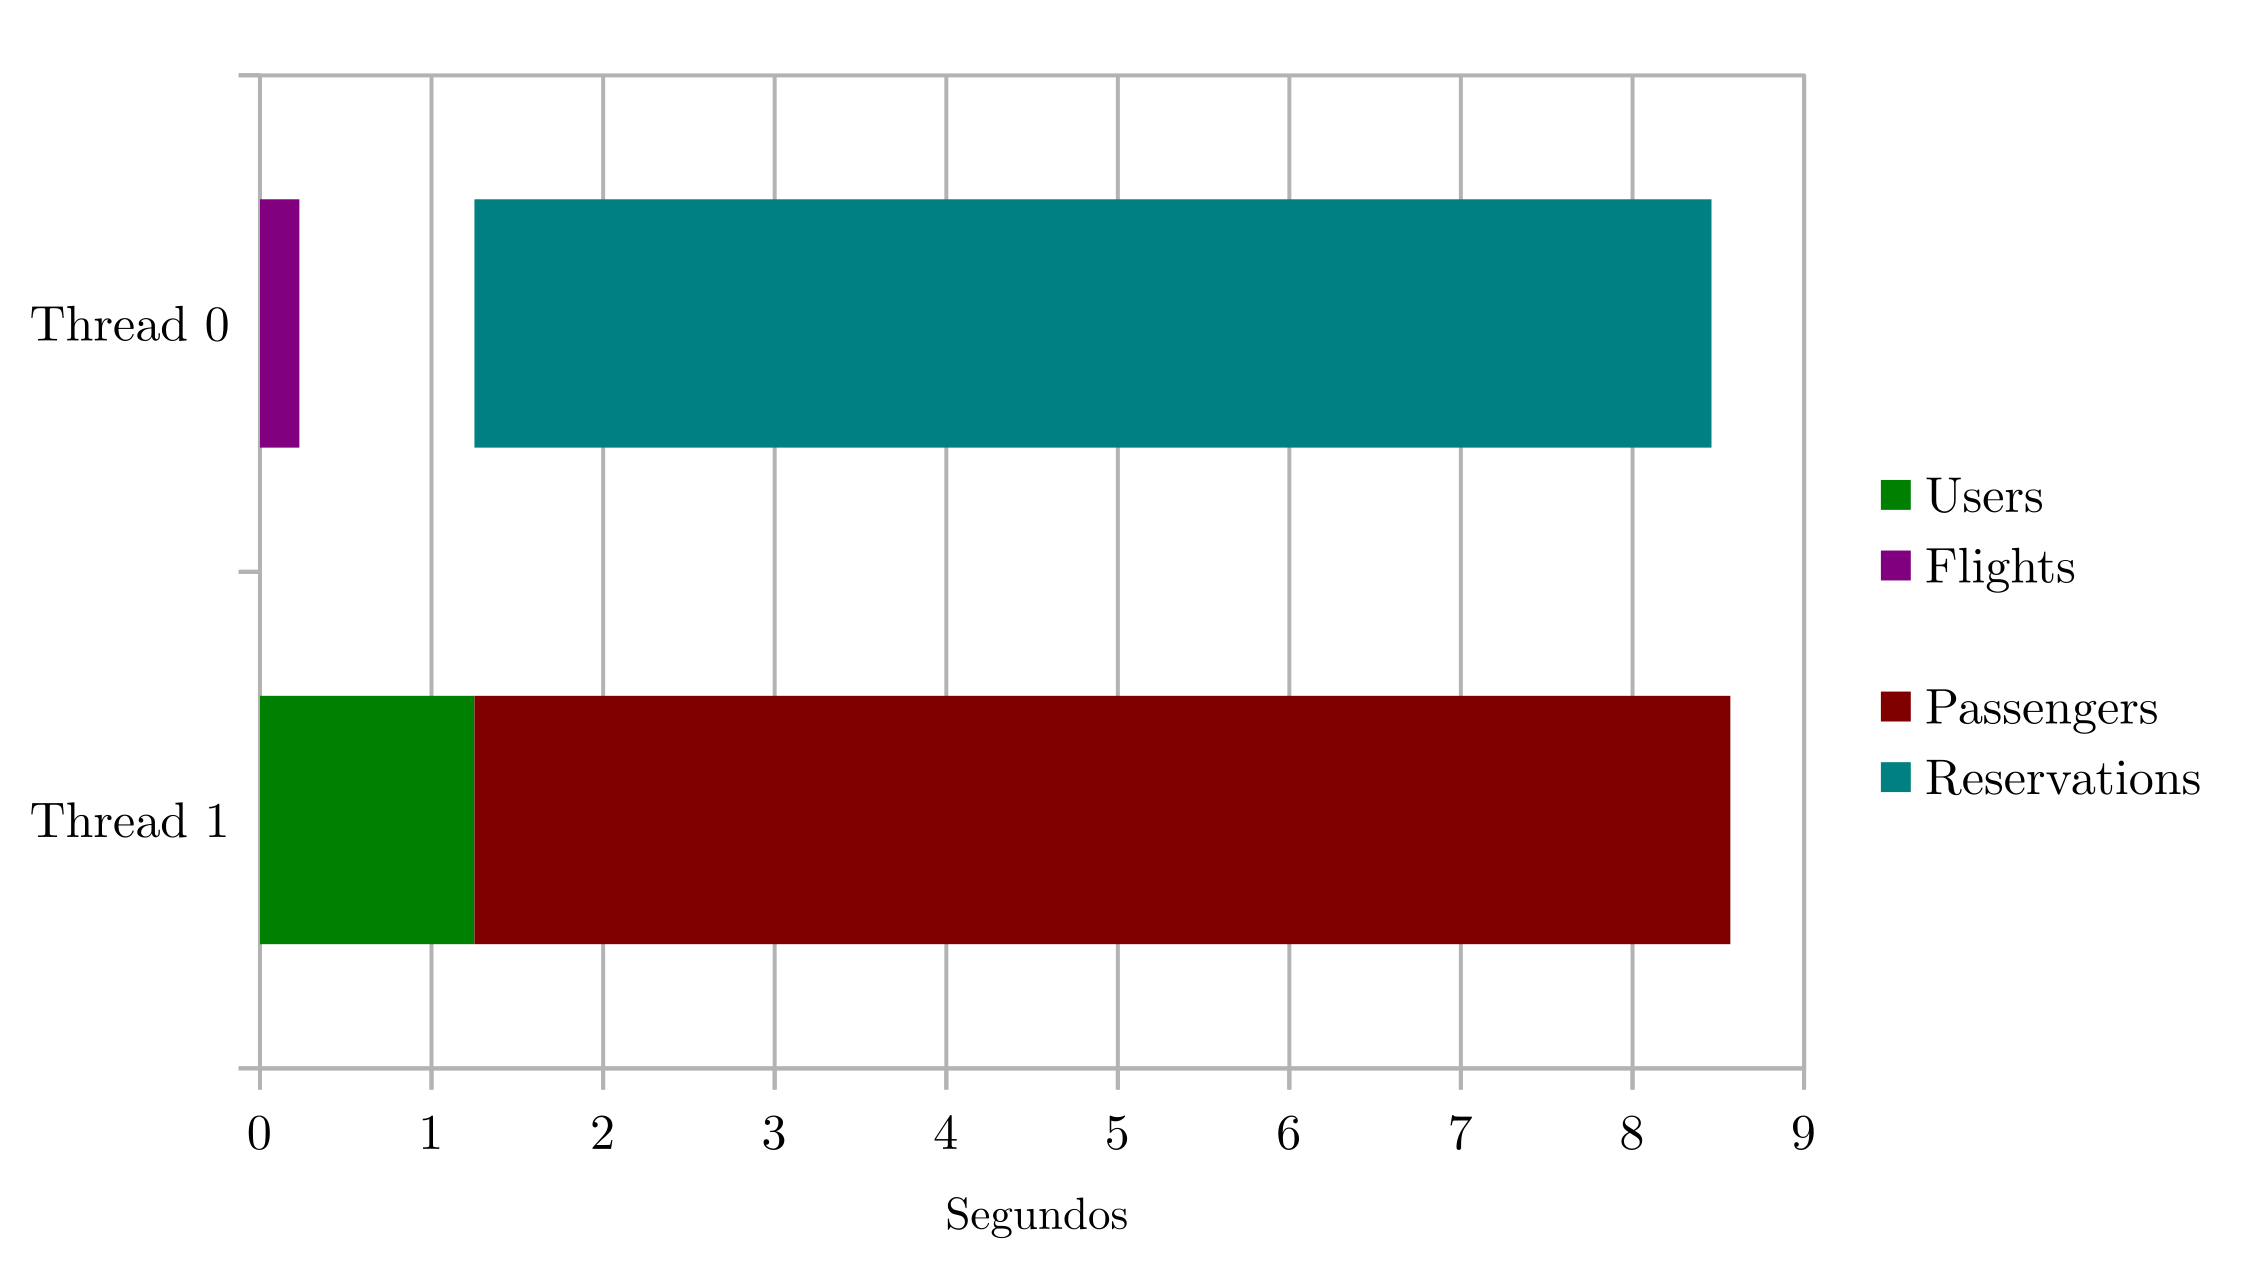
\includegraphics[scale=0.20]{res-fase2/threading.png}
    \caption{Possível distribuição de tarefas por \emph{threads}, com os tempos da
             \hyperref[fig:dataset-screenshot]{Figura \ref*{fig:dataset-screenshot}}}
    \label{fig:threading}
\end{figure}

A distribuição de tarefas acima cumpre as condições necessárias para assegurar as relações de
dependência de dados (reservas depois dos utilizadores, passageiros depois dos utilizadores e dos
voos) e consegue reduzir o tempo de \emph{parsing} de 16 s para um mínimo teórico de 8.6 s! A única
dependência de dados que encontrámos, um alocador, é facilmente resolúvel com o uso de dois
alocadores distintos para as relações utilizador -- voo / reserva.

\section{Conclusão}
\label{sec:conclusion}

Estamos bastante satisfeitos com o resultado final deste trabalho, onde pudemos aplicar
conhecimentos de várias UCs. Pensamos que a maior conclusão a tirar deste projeto seja a importância
de se pensar bastante antes de se escrever qualquer programa. Esta filosofia aplica-se ao
desenvolvimento de aplicações modulares e encapsuladas, à escolha da \emph{schema} de uma base de
dados para o melhor desempenho, à arquitetura global de um programa para este ser facilmente
extensível, \emph{etc.} O desenvolvimento destes 75 módulos permitiu-nos aprofundar o nosso
conhecimento em C, o que por sua vez nos capacitou para implementar conceitos de outras linguagens e
paradigmas, para suprir certas lacunas de C: polimorfismo, tipos genéricos, alocadores customizados,
\emph{etc.}

\pagebreak
\section{Anexos}
\label{sec:annexes}

\subsection{\emph{Screenshots} do modo interativo}
\label{sec:interactive-screenshots}

\begin{figure}[H]
    \centering
    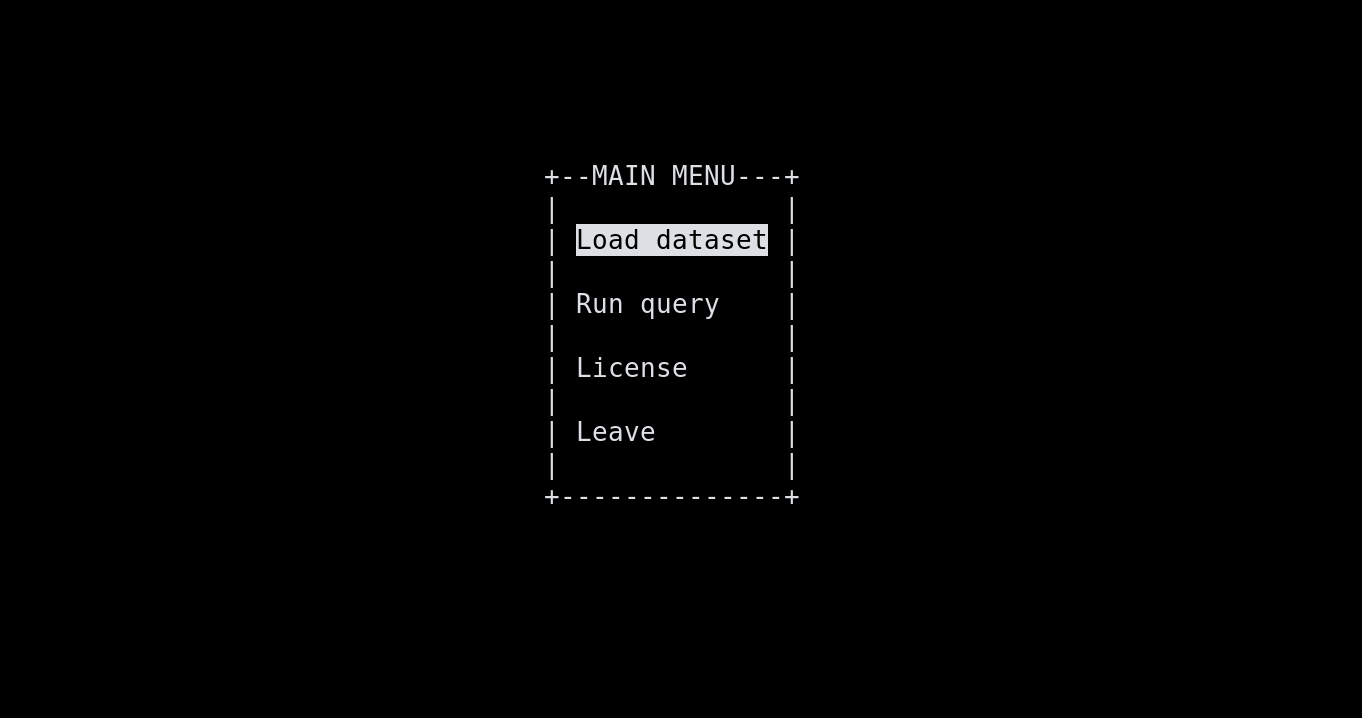
\includegraphics[scale=0.25]{res-fase2/interactive_screenshots/main_menu.png}
    \caption{Menu (\texttt{activity\_menu}), em particular, o menu principal
             (\texttt{activity\_main\_menu})}
    \label{fig:main_menu}
\end{figure}

\begin{figure}[H]
    \centering
    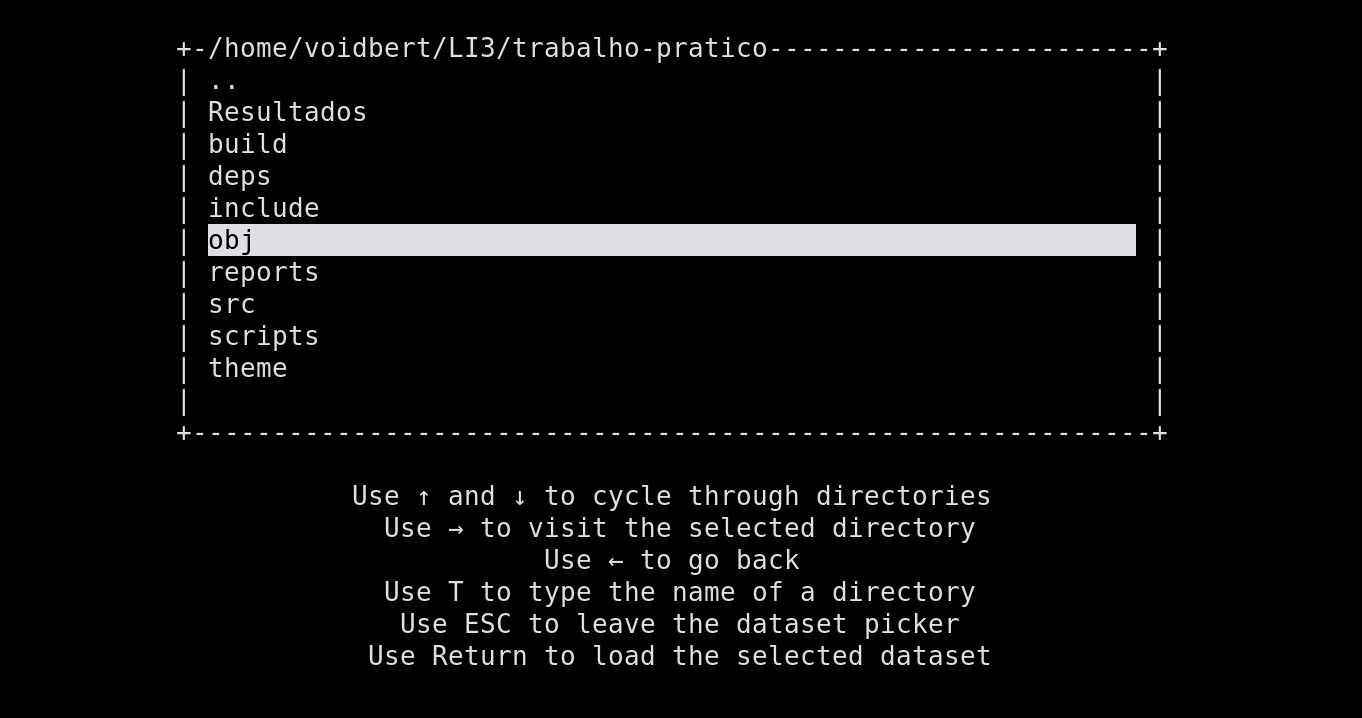
\includegraphics[scale=0.25]{res-fase2/interactive_screenshots/dataset_picker.png}
    \caption{Navegador de ficheiros para a escolha de um \emph{dataset}
             (\texttt{activity\_dataset\_picker})}
    \label{fig:dataset_picker}
\end{figure}

\begin{figure}[H]
    \centering
    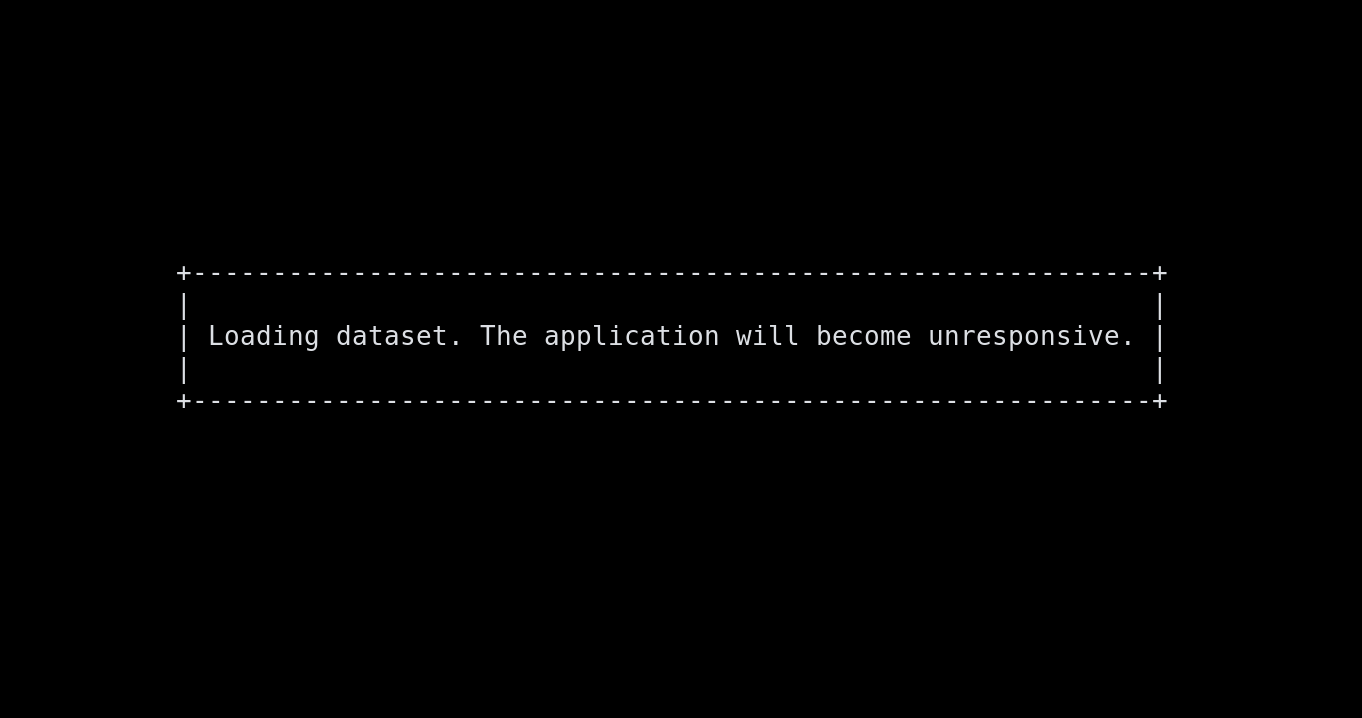
\includegraphics[scale=0.25]{res-fase2/interactive_screenshots/loading_dataset.png}
    \caption{Ecrã durante a leitura de um \emph{dataset} (\texttt{screen\_loading\_dataset})}
    \label{fig:loading_dataset}
\end{figure}

\begin{figure}[H]
    \centering
    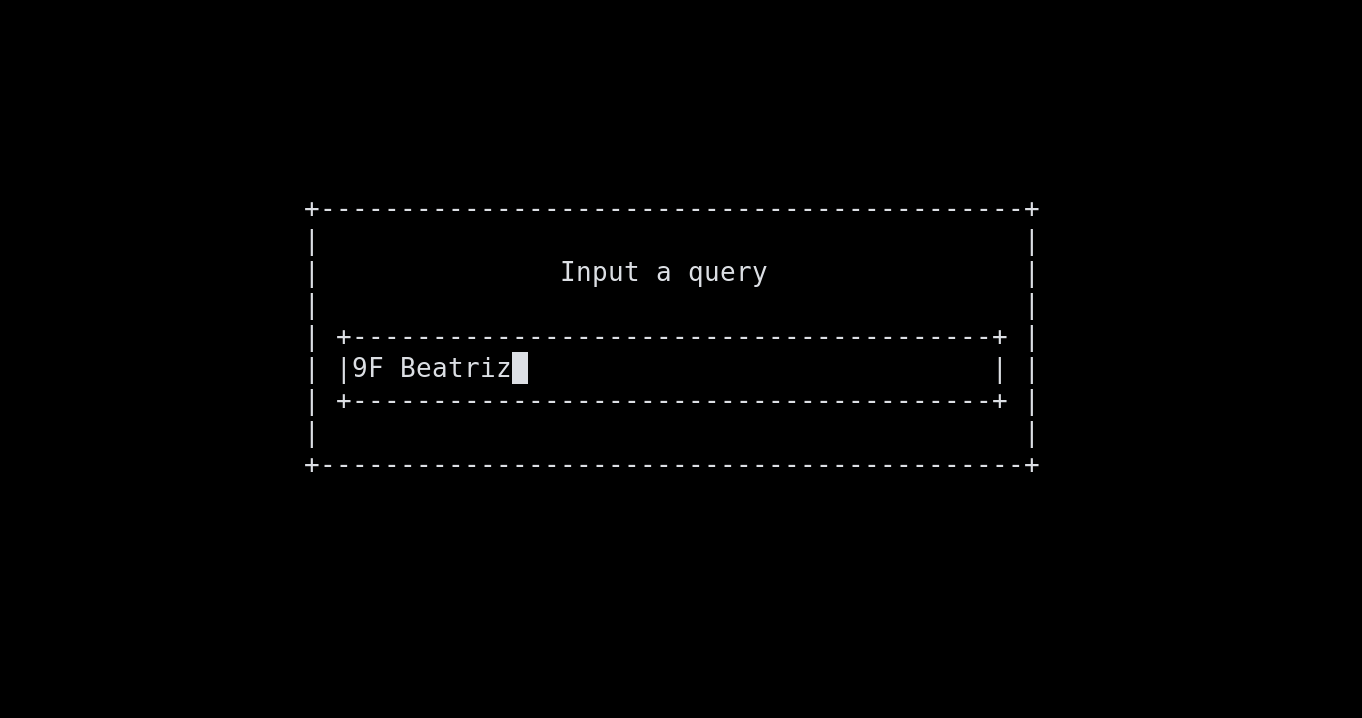
\includegraphics[scale=0.25]{res-fase2/interactive_screenshots/textbox.png}
    \caption{Caixa de texto para a entrada de uma \emph{query} (\texttt{activity\_textbox})}
    \label{fig:textbox}
\end{figure}

\begin{figure}[H]
    \centering
    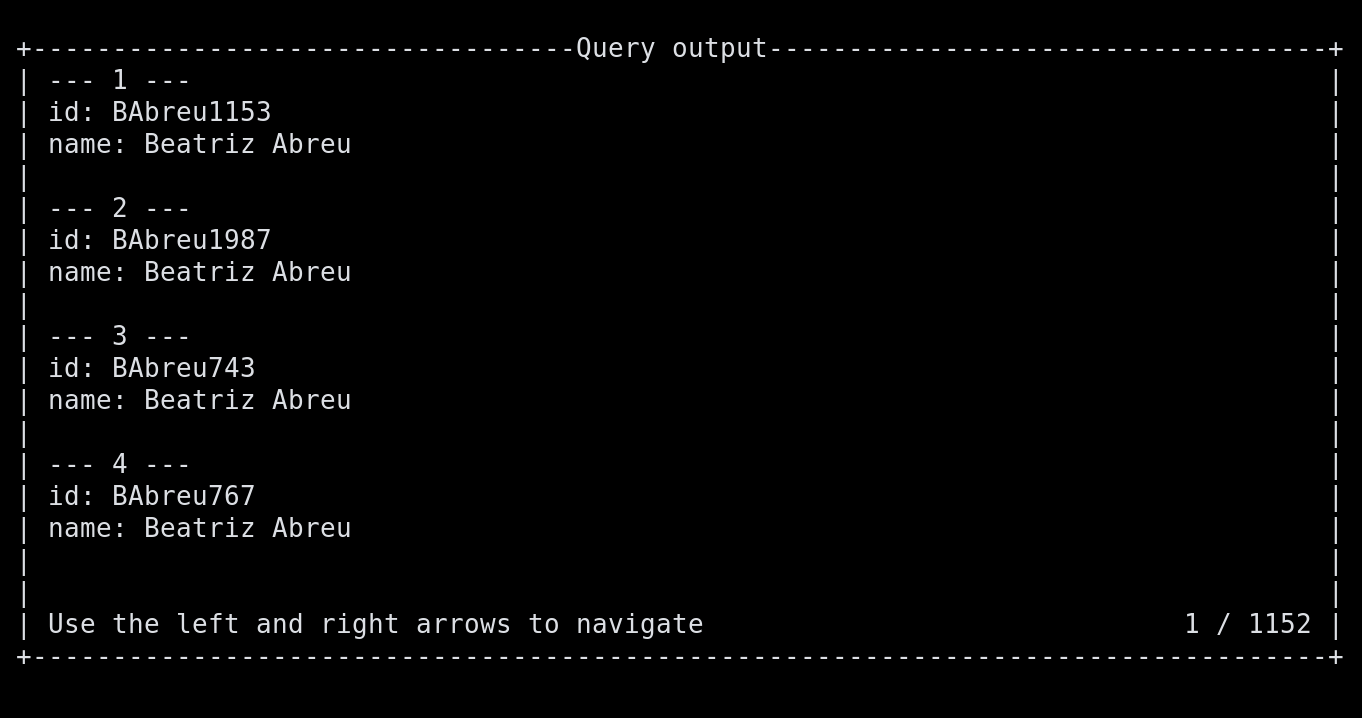
\includegraphics[scale=0.25]{res-fase2/interactive_screenshots/paging.png}
    \caption{Output paginado de uma \emph{query} (\texttt{activity\_paging})}
    \label{fig:paging}
\end{figure}

\begin{figure}[H]
    \centering
    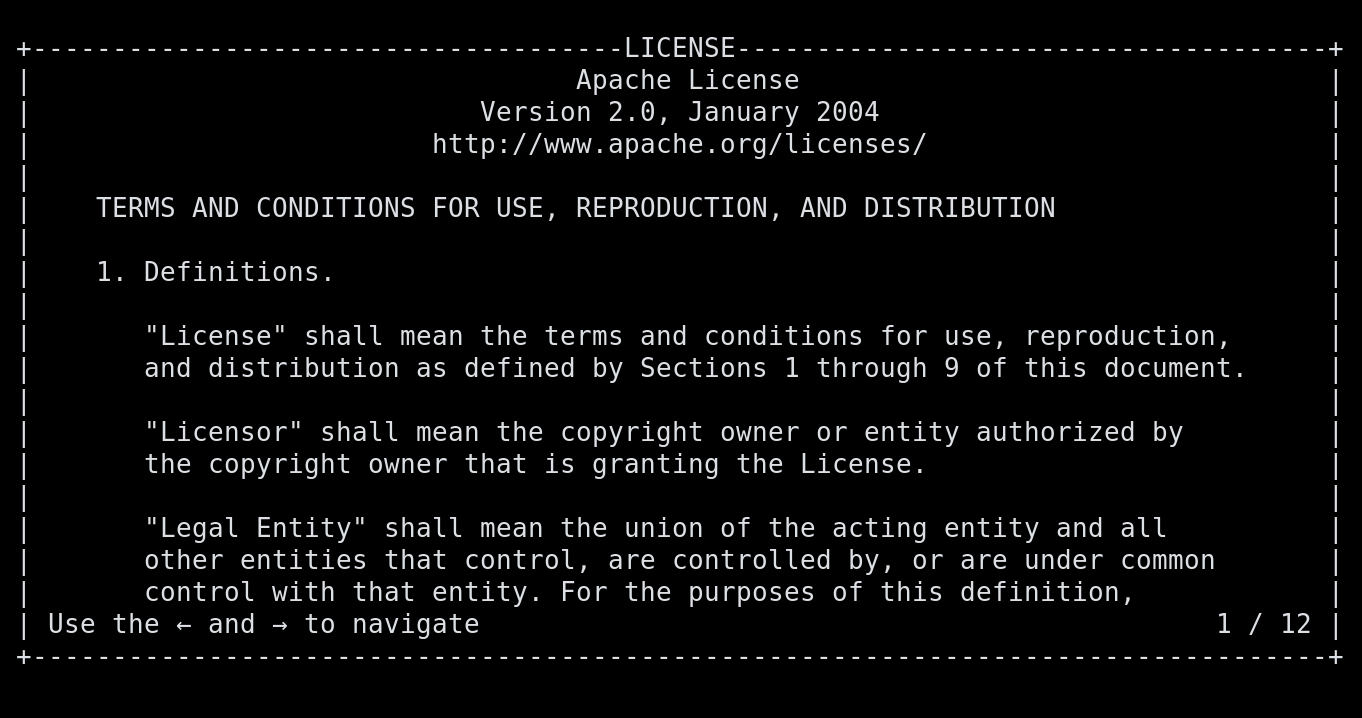
\includegraphics[scale=0.25]{res-fase2/interactive_screenshots/license.png}
    \caption{Licença da aplicação (\texttt{activity\_license})}
    \label{fig:license}
\end{figure}

\begin{figure}[H]
    \centering
    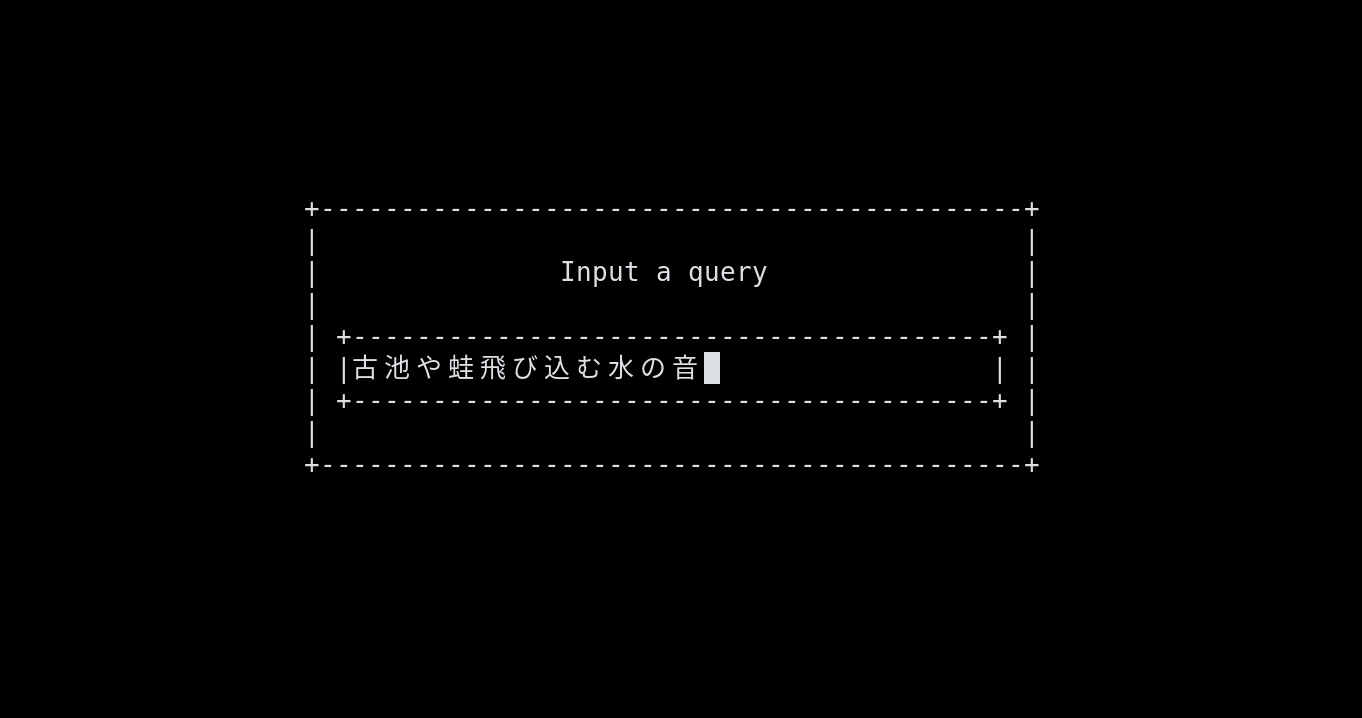
\includegraphics[scale=0.25]{res-fase2/interactive_screenshots/japanese.png}
    \caption{Suporte para caracteres de largura dupla numa \texttt{activity\_textbox}.
             O \emph{scrolling} mantém-se funcional.}
    \label{fig:japanese}
\end{figure}

\begin{figure}[H]
    \centering
    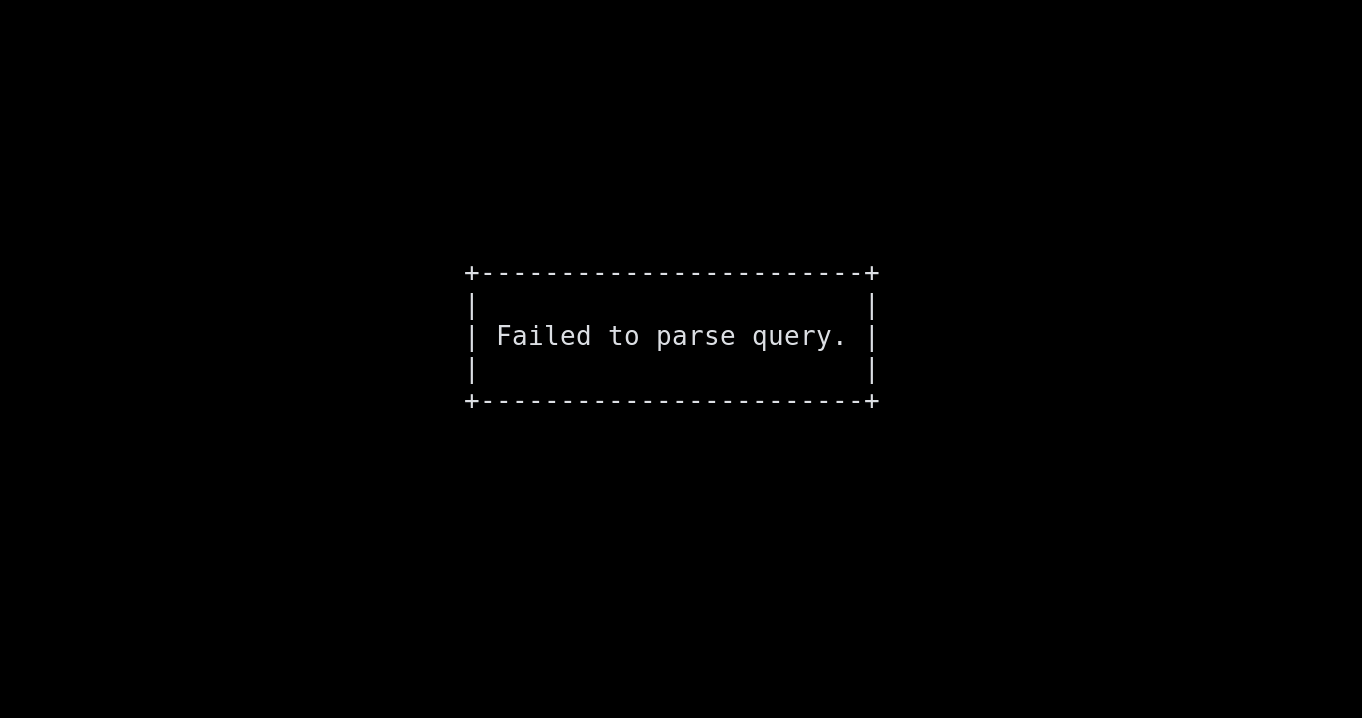
\includegraphics[scale=0.25]{res-fase2/interactive_screenshots/messagebox.png}
    \caption{Aviso de erro numa \texttt{activity\_messagebox}}
    \label{fig:messagebox}
\end{figure}

\subsection{\emph{Screenshots} do \emph{output} dos testes}
\label{sec:testing-screenshots}

\begin{figure}[H]
    \centering
    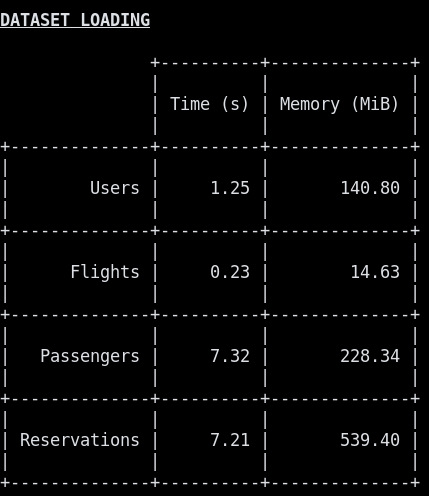
\includegraphics[scale=0.4]{res-fase2/testing_screenshots/dataset.png}
    \caption{Tabela de tempos de leitura de cada parte de um \emph{dataset}}
    \label{fig:dataset-screenshot}
\end{figure}

\begin{figure}[H]
    \centering
    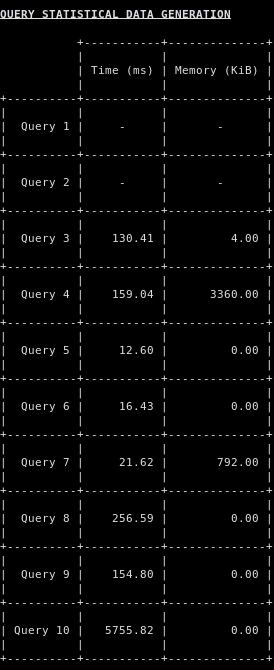
\includegraphics[scale=0.6]{res-fase2/testing_screenshots/statistics.png}
    \caption{Tabela de tempos de geração de dados estatísticos para cada \emph{query}}
    \label{fig:query-screenshot}
\end{figure}

\begin{figure}[H]
    \centering
    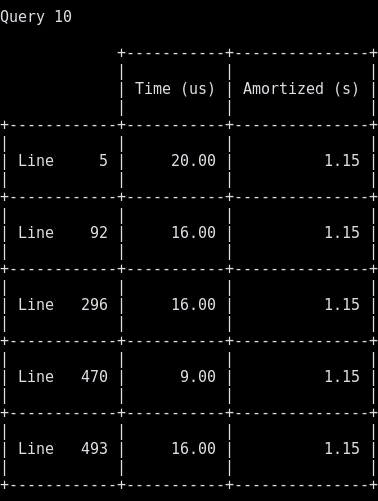
\includegraphics[scale=0.5]{res-fase2/testing_screenshots/query.png}
    \caption{Tabela de tempos de execução de cada \emph{query}. É visível como são automaticamente
             escolhidas duas unidades diferentes para as duas colunas.}
    \label{fig:q10-screenshot}
\end{figure}

\begin{figure}[H]
    \centering
    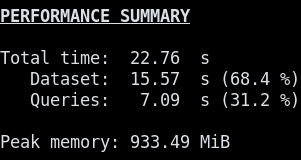
\includegraphics[scale=0.7]{res-fase2/testing_screenshots/summary.png}
    \caption{Sumário do \emph{benchmarking} da aplicação}
    \label{fig:performance-summary}
\end{figure}

\begin{figure}[H]
    \centering
    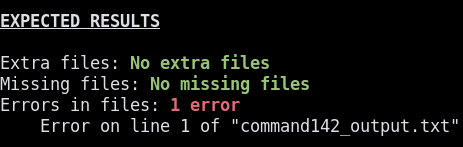
\includegraphics[scale=0.6]{res-fase2/testing_screenshots/diff.png}
    \caption{Exemplo de resultado de testes funcionais com um erro}
    \label{fig:diff-screenshot}
\end{figure}

\end{document}
